\documentclass[a4paper, 10pt]{article}
\usepackage[UTF8]{ctex}
\usepackage{geometry}
\usepackage{indentfirst}
\usepackage{amsmath}
\usepackage{amssymb}
\usepackage{graphicx}
\usepackage{subfigure}
\usepackage{enumerate}
\usepackage{listings}
\usepackage{appendix}
\usepackage{xcolor}
% \usepackage[table,xcdraw]{xcolor}
\usepackage{hyperref}
\hypersetup{colorlinks=true,linkcolor=black}
\usepackage{framed}
\usepackage{multirow}
\usepackage{algorithm}
\usepackage{algorithmicx}
\usepackage{algpseudocode}
\usepackage{amsmath}
\renewcommand{\algorithmicrequire}{\textbf{Input:}}
\renewcommand{\algorithmicensure}{\textbf{Output:}}
\lstset{
    numbers=left,
    numberstyle= \tiny,
    keywordstyle= \color{ blue!70},
    commentstyle= \color{red!50!green!50!blue!50},
    frame=shadowbox,
    rulesepcolor= \color{ red!20!green!20!blue!20} ,
    escapeinside=``,
    xleftmargin=1em,xrightmargin=0em, aboveskip=1em,
    framexleftmargin=2em,
    showstringspaces=false,
    showtabs=false,
    breaklines=true
}

\title{大作业报告——诗歌搜索引擎}
\author{戴昊悦\quad 王中烨\quad 李竞宇\quad 陈浩平}

\begin{document}

\maketitle
\tableofcontents
\newpage

\section{项目综述}
读诗是一种美好的享受。但目前网络上的诗歌库,比如中国诗歌网、古诗文网等,要么是数据量较小,要么是表单样式的网站,没有丰富的功能。我们希望将诗歌用一种更好的形式展现给用户,因此利用本学期电工导知识实现了此诗歌引擎:Poem Inspire。

我们的引擎数据量涵盖了全部诗经、唐宋古诗30万余首、宋词元曲等2万余首、中文现代诗5千余首、英文现代诗1万余首、诗歌配图约18万张、赏析5千余篇,以及相应的2万余名诗人信息、1万余个标签。

我们的搜索引擎采用Bootstrap作为前端的框架,利用Javascript实现了与模型有关的部分的前后端的异步交互,避免页面的加载时间过长。我们的搜索引擎后端利用web.py实现对网页前端的支持,使用高效的elastic-search实现数据的索引和搜索。

我们使用额外数据和词频分析建立了现代诗和古诗的词典和TF-IDF词典,并借助jieba的有关功能实现了现代诗和古诗文的文本分析和关键词抽取。我们使用深度卷积神经网络实现了图片到物象的转化以及建立图片与诗歌间的联系从而实现为诗歌配图、由图片搜索和生成现代诗和古诗文。

我们实现的功能具体包括包括:
\begin{itemize}
\setlength{\itemsep}{0pt}
\setlength{\parsep}{0pt}
\setlength{\parskip}{0pt}
    \item \textbf{信息整合}:对每首诗提供信息页面,包括正文、作者、意象、标签、年代、自动配图,有助于读者对一首诗产生直观印象;
    \item \textbf{分类查看}:对作者、流派、标签等制作专门页面,方便用户阅读研究该类别下的诗歌;
    \item \textbf{模糊搜索}:将用户的输入对标题、正文、赏析等多个搜索域进行搜索,展现全面的内容;
    \item \textbf{精确搜索}:集成在在高级搜索的多个选择框内,用户可指定对某类诗的某个域搜索;
    \item \textbf{词义联想}:考虑到用户输入现代汉语与古诗词的差异性,我们实现了古词联想,比如输入“酒店”,联想到“逆旅 酒楼 客舍 酒肆 旅亭 馆驿 帆宿 客馆 酒家 炊烟 厨香 杏花村...”;
    \item \textbf{自动配图}:用户输入某首诗,将分析其表达的意象,并返回主题最适合的配图;
    \item \textbf{以图搜诗}:用户上传一张图片,将分析图片包含的物体、场景、情感信息,搜索返回与图片最相符合的诗歌;
    \item \textbf{以图写诗}:用户上传一张图片,并可以自由选择特征信息,自动从图片生成现代诗、绝句及律诗。
    \item \textbf{每日推荐}:主页每日推荐,包括横幅诗图、古诗现代诗推荐、标签推荐等;
\end{itemize}

在本报告中,我们将首先简要的展示我们的搜索引擎成果,然后依次介绍我们是如何获取数据、建立索引、实现网站的,最后我们将着重介绍在我们搜索引擎中的图片-诗歌生成模型。


\section{成果展示}
在此节中,我们将简要展示我们的搜索引擎的页面和功能。

\paragraph*{首页推荐} 图\ref{fig:landing1}和\ref{fig:landing2}所示为我们搜索引擎的首页,其中包含了每日自动更新的推荐内容,和每次刷新都会更新的诗歌推荐内容。推荐的具体算法可以通过浏览器的Cookie取回用户的常用搜索关键词进行相似度推荐,或利用用户浏览的诗歌进行关联推荐。由于时间原因,我们未能着手实现推荐算法,目前使用随机取回诗歌填充推荐的内容。对于每日推荐,将当天日期作为随机数种子,定义相应变量保存诗歌id信息,每天更新一次。每日一诗由于位于页首,背景为其配图,限于篇幅,对其正文长度限制在50字以内,对不符合要求的诗歌进行线性搜索。页面最后列出了这些诗歌对应的标签,方便用户点击查询。

\begin{figure}[H]
\centering
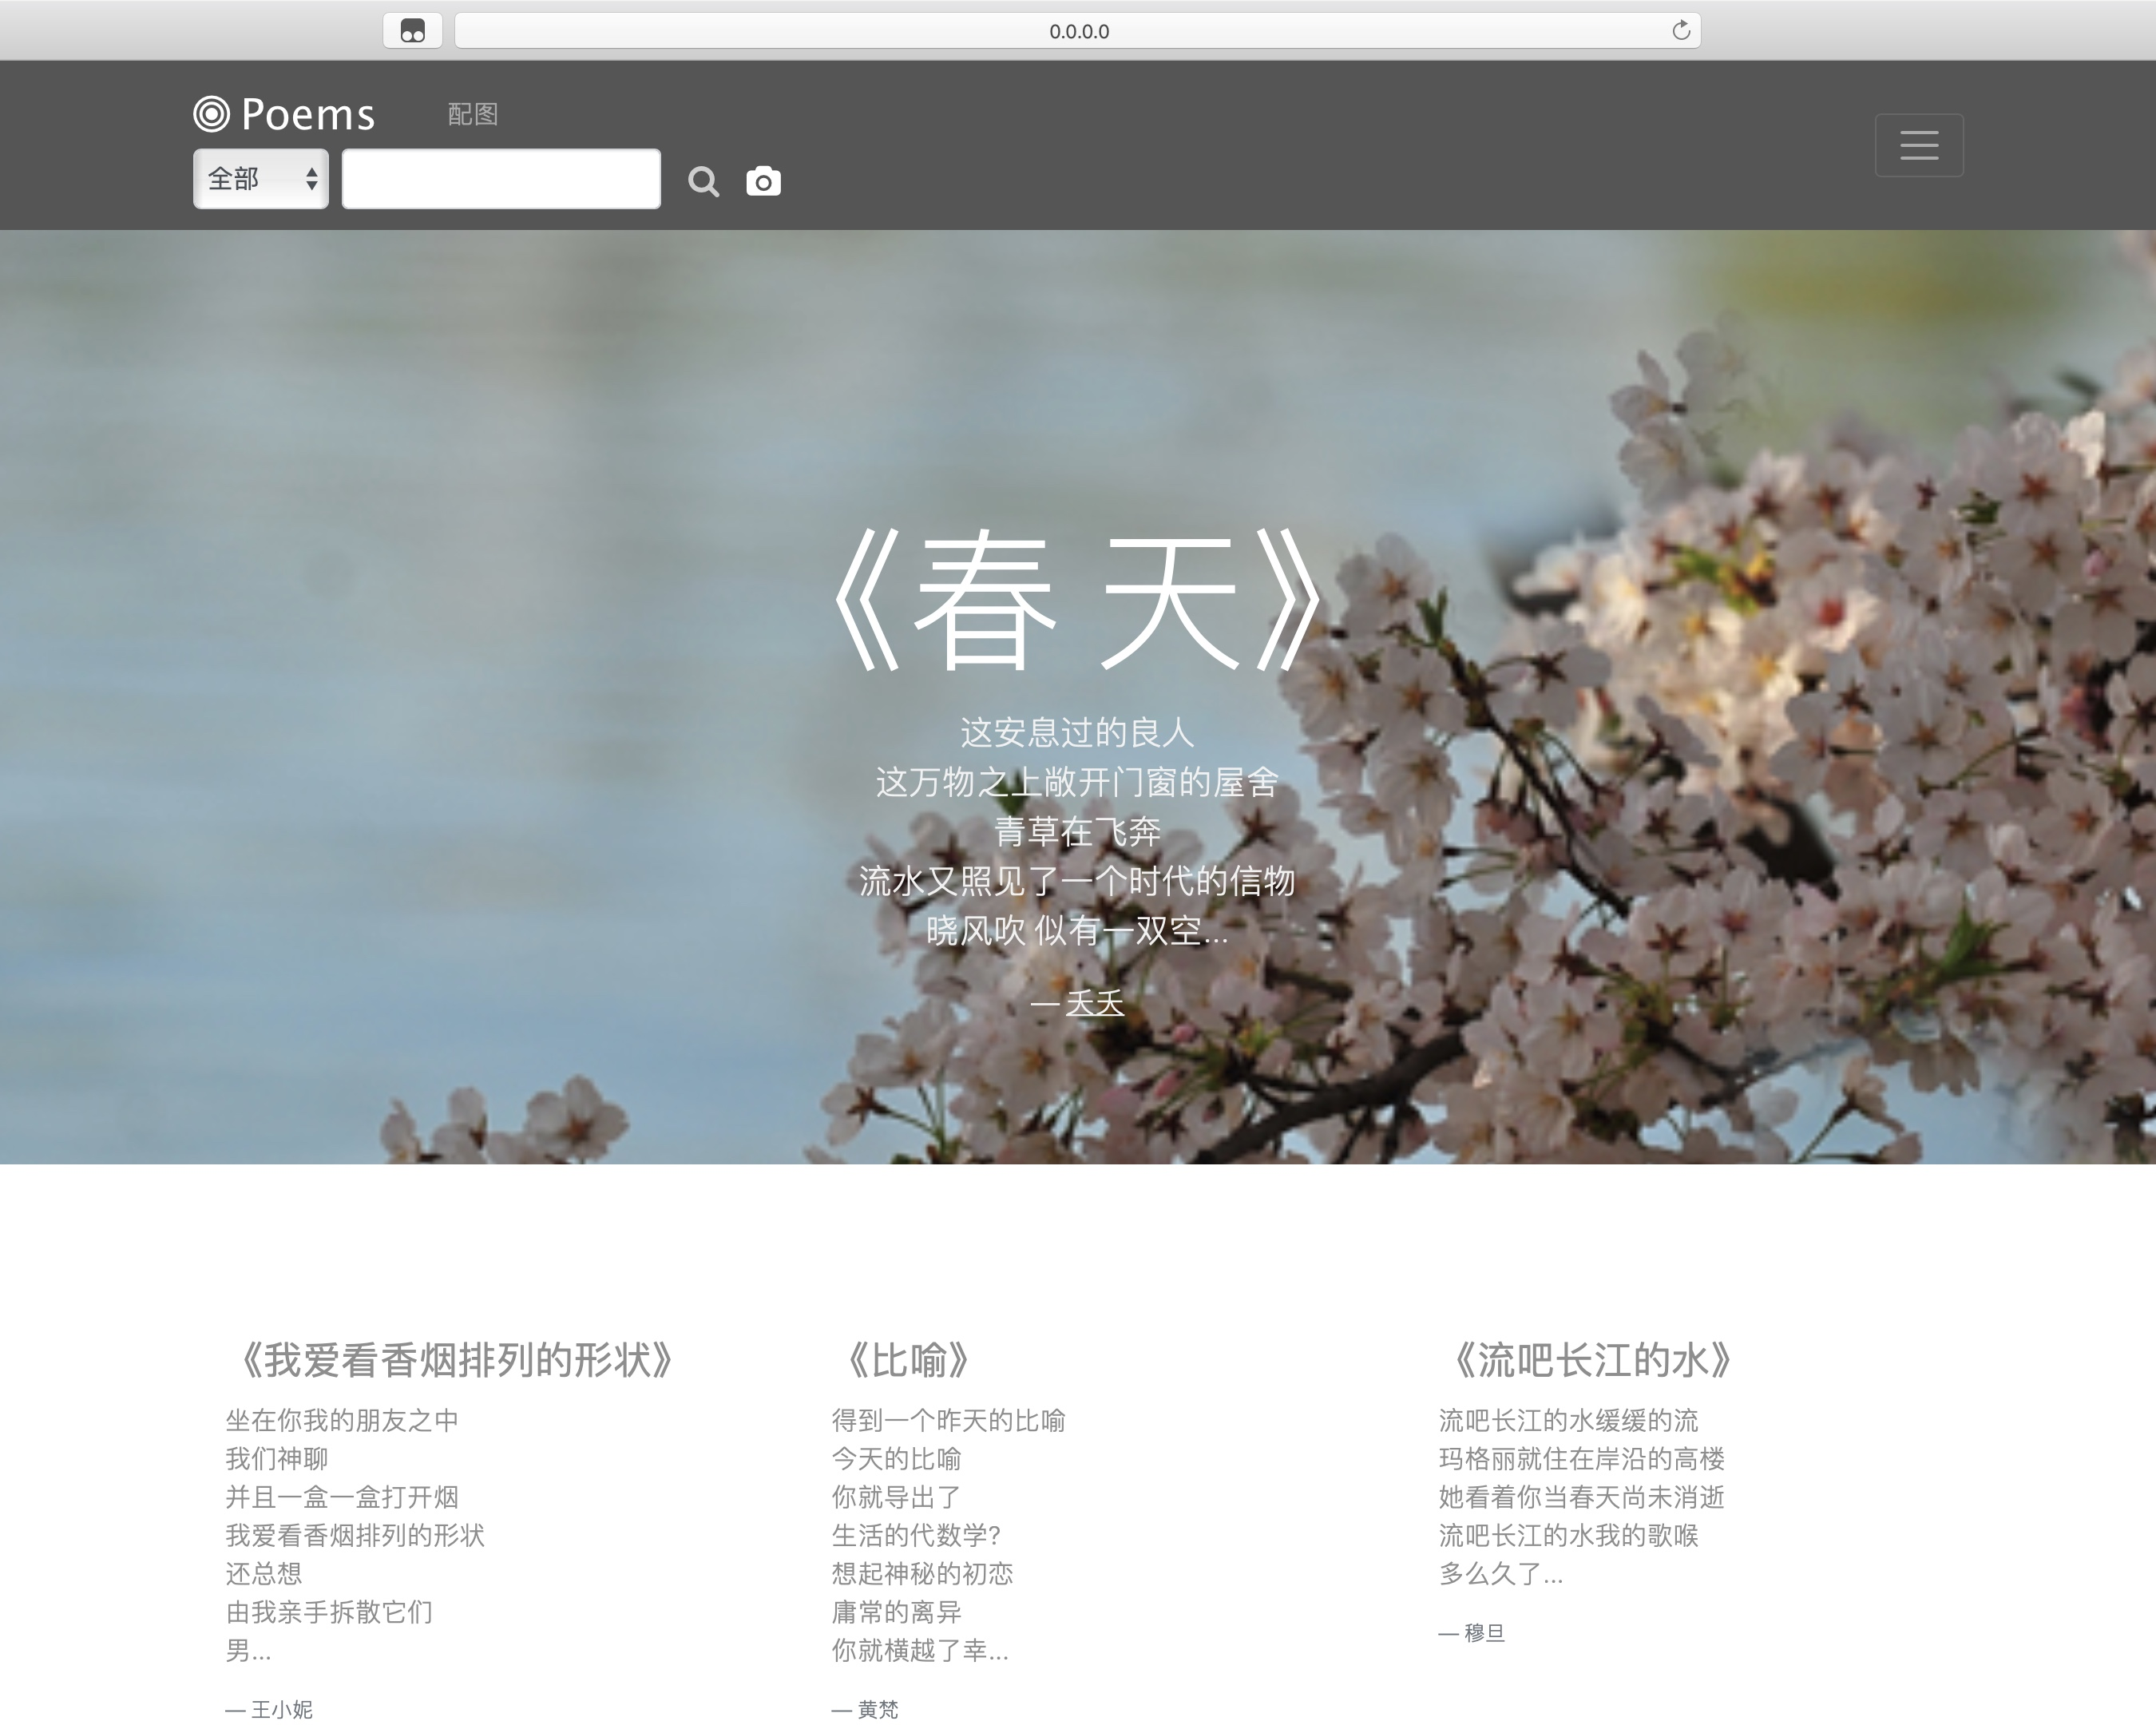
\includegraphics[width=1.0\linewidth]{fig/landing1.jpg}
\caption{每日一诗}
\label{fig:landing1}
\end{figure}
\begin{figure}[H]
\centering
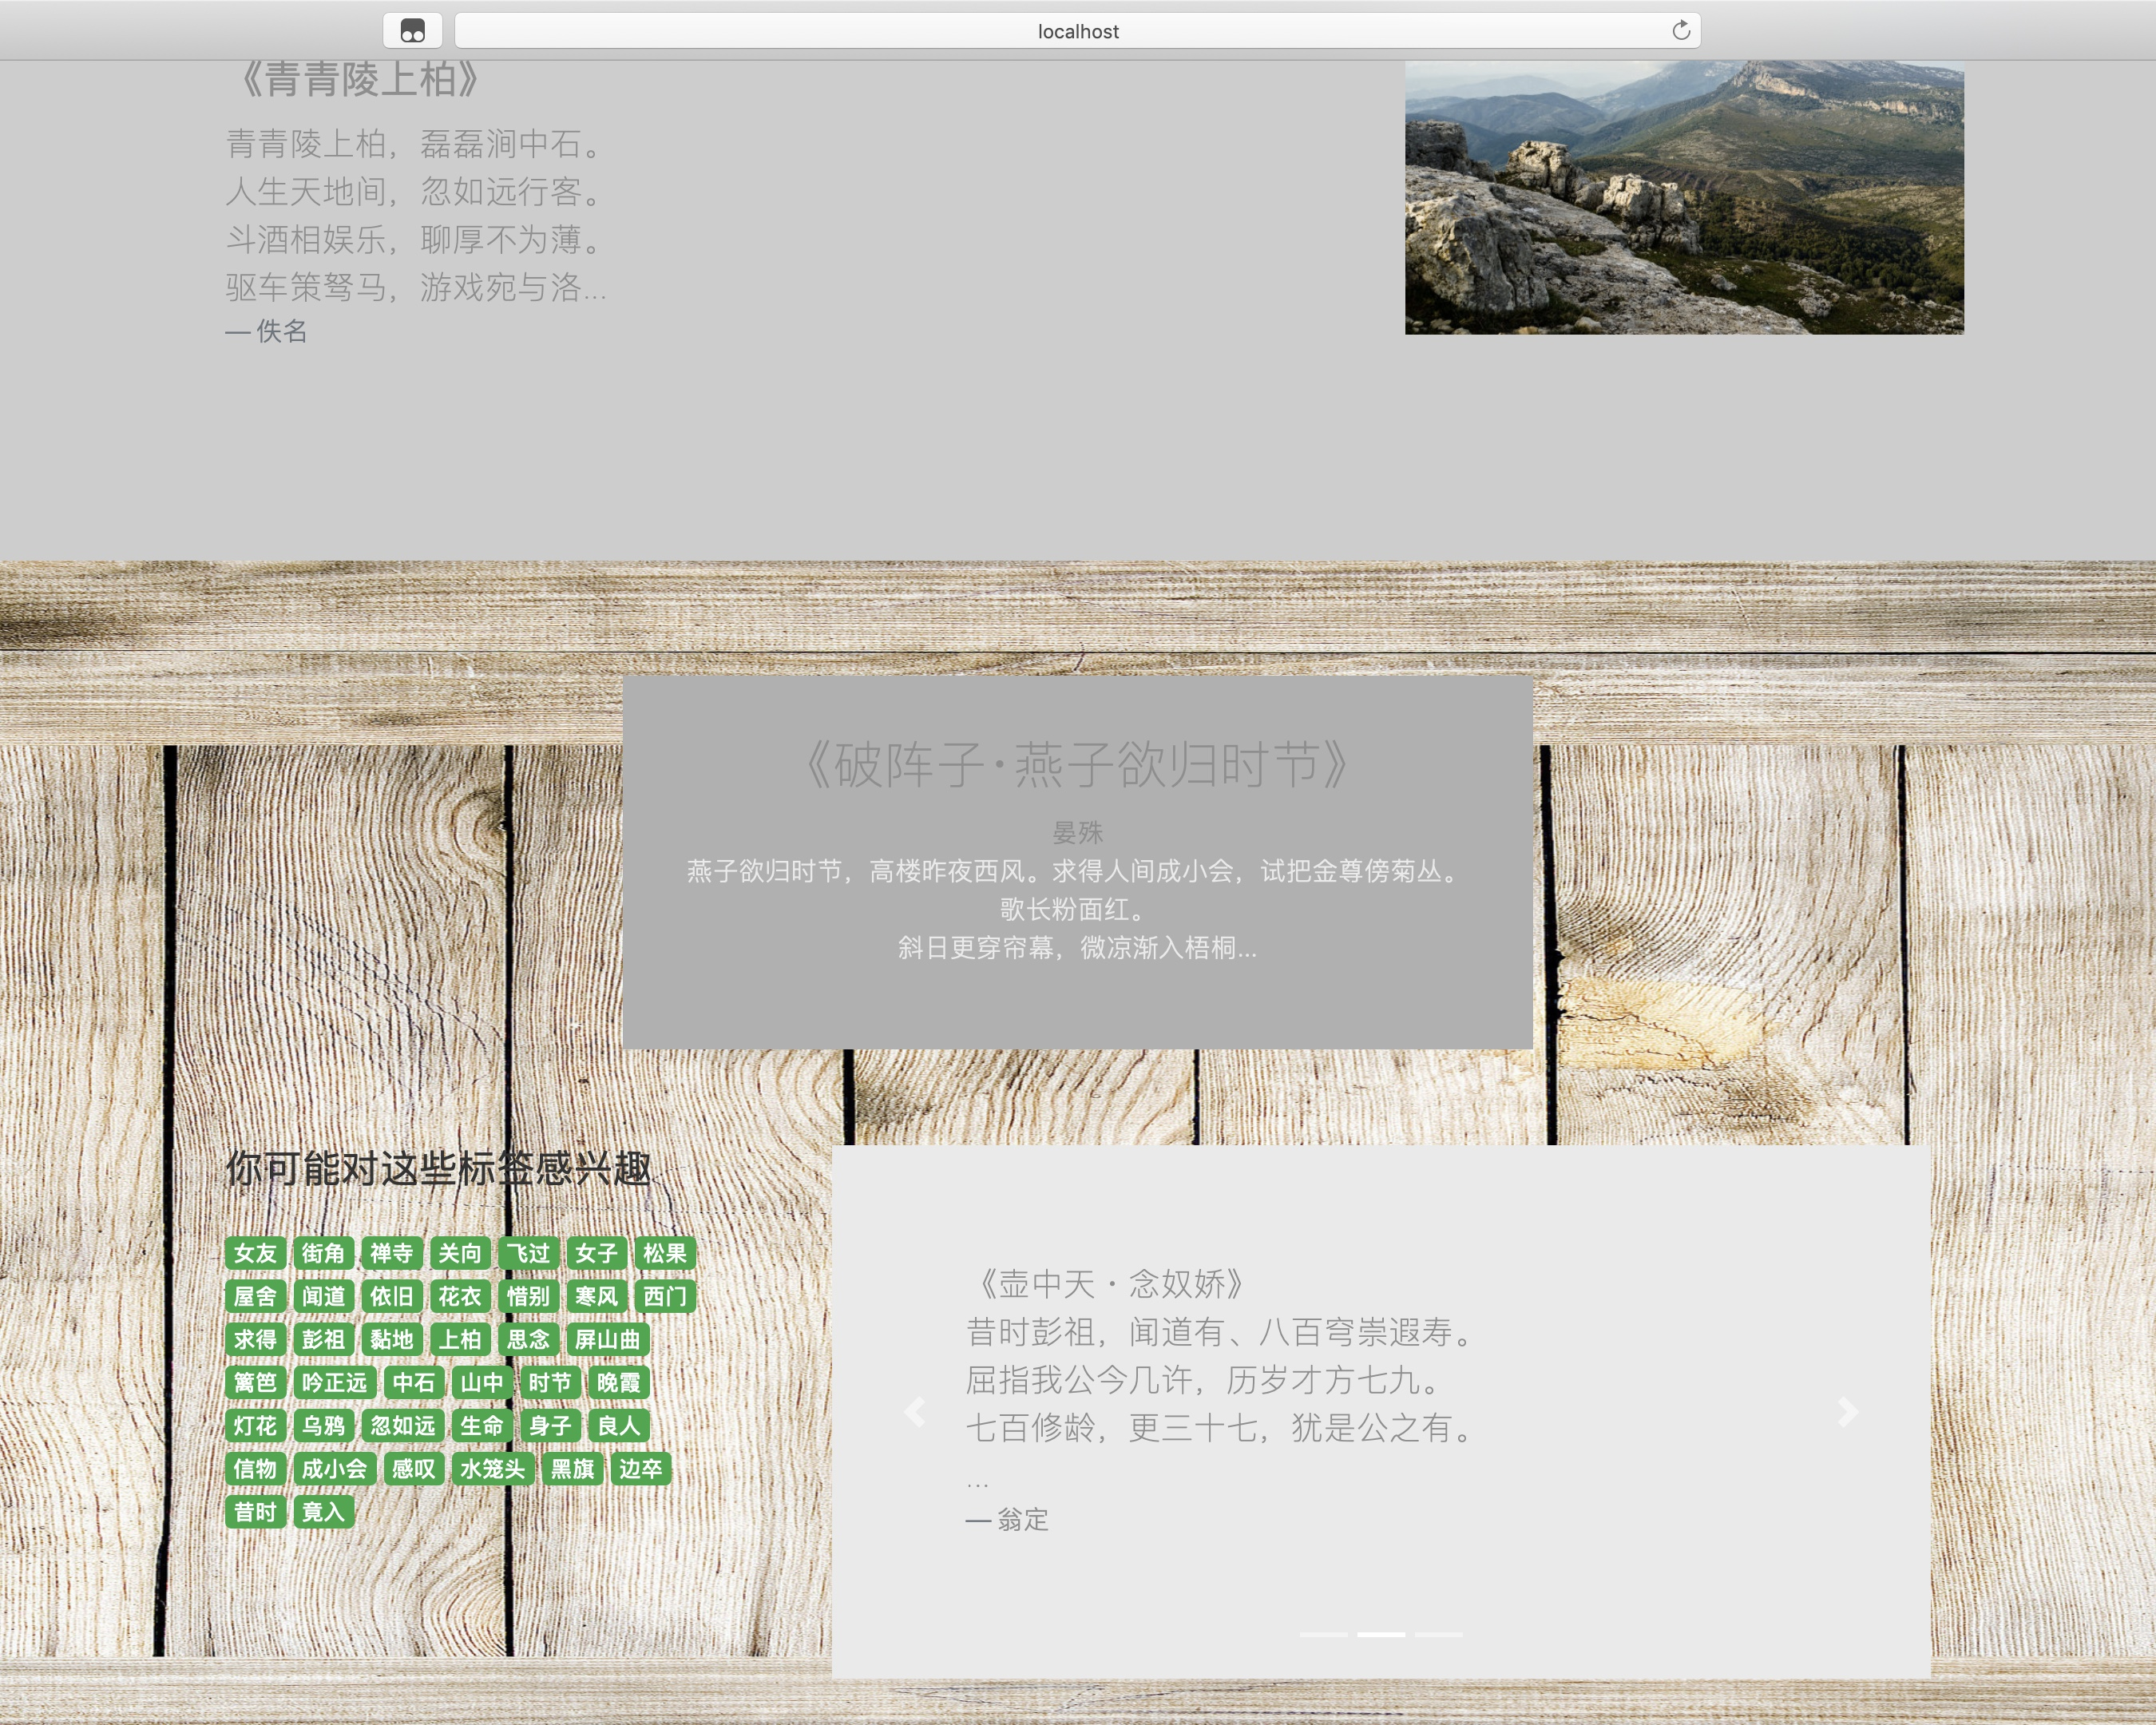
\includegraphics[width=1.0\linewidth]{fig/landing2.jpg}
\caption{首页推荐}
\label{fig:landing2}
\end{figure}

\paragraph*{搜索接口} 作为一个搜索引擎,其最核心的页面要素便是搜索接口。图\ref{fig:demo_searchbar}所示为我们搜索引擎提供给用户的接口,该接口在网页所有页面都存在。该搜索表单嵌入在页面的导航栏中,默认情况下收起高级搜索表单,仅显示搜索诗歌的类型(全部、现代诗、古诗文)和模糊搜索输入框,展开后用户可以自定义当前的查询细节。

\begin{figure}[H]
\centering
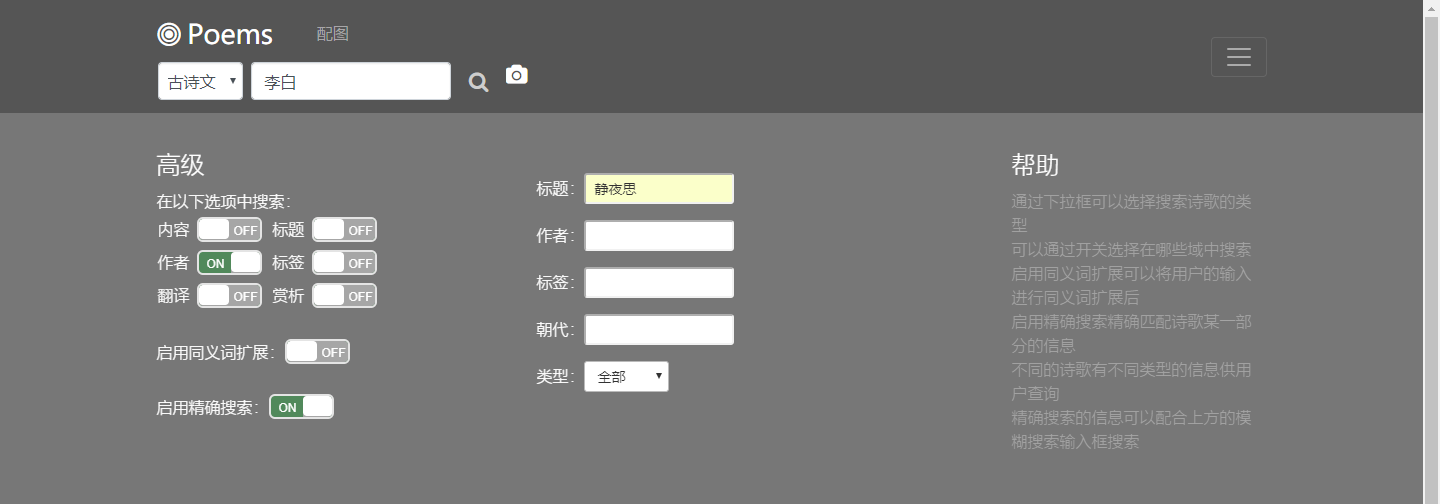
\includegraphics[scale=0.5]{fig/demo_searchbar.png}
\caption{搜索接口}
\label{fig:demo_searchbar}
\end{figure}

首先,我们允许用户选择在哪些域中进行模糊搜索。打开相应的开关可以另当前查询包括相应的域,有多个域被选择后,搜索引擎将返回匹配尽可能多的域的结果。翻译和赏析仅对古诗文搜索类型有效。如果所有域都被关闭,当前查询会被归类为无效查询并反馈相应信息给用户。网页默认开启所有的搜索域。

其次,我们提供同义词扩展功能。当用户对查询的关键词不确定时,可以开启这一功能,搜索引擎将会利用内置的词库对查询中的每个词进行同义词扩展,扩大搜索结果的覆盖范围,提高用户找到所希望得到的结果。这一功能仅对在内容中搜索的查询进行扩展。

最后,我们提供精确查询接口,让用户进一步明确当前查询的细节。对于不同的查询类型,我们提供不同的搜索域。对于古诗文,用户可以明确诗歌的标题、作者、标签、朝代或类型(诗、词、曲等);对于现代诗,用户可以明确诗歌的标题、作者、标签、流派或年代。如果一个域在精确搜索中被使用,该域中的搜索将不会使用模糊搜索框中的字段。

图\ref{fig:demo_searchbar}中所示的样例查询仅在作者域中模糊搜索“李白”这一字段,不使用同义词扩展,在标题域中精确搜索“静夜思”这一字段。其余字段为空将不对它们进行精确搜索。

除此之外,用户还可点击搜索按钮边上的相机按钮,上传希望分析并用于搜索诗歌的图片。用户还可通过上方的链接跳转至配图页面,上传自创的诗歌并为之匹配合适的图片。


\paragraph*{结果页面} 图\ref{fig:demo_accres}所示为上述查询的搜索结果,可见搜索引擎精确的返回了一条作者是李白,诗名为《静夜思》的诗歌。

\begin{figure}[H]
\centering
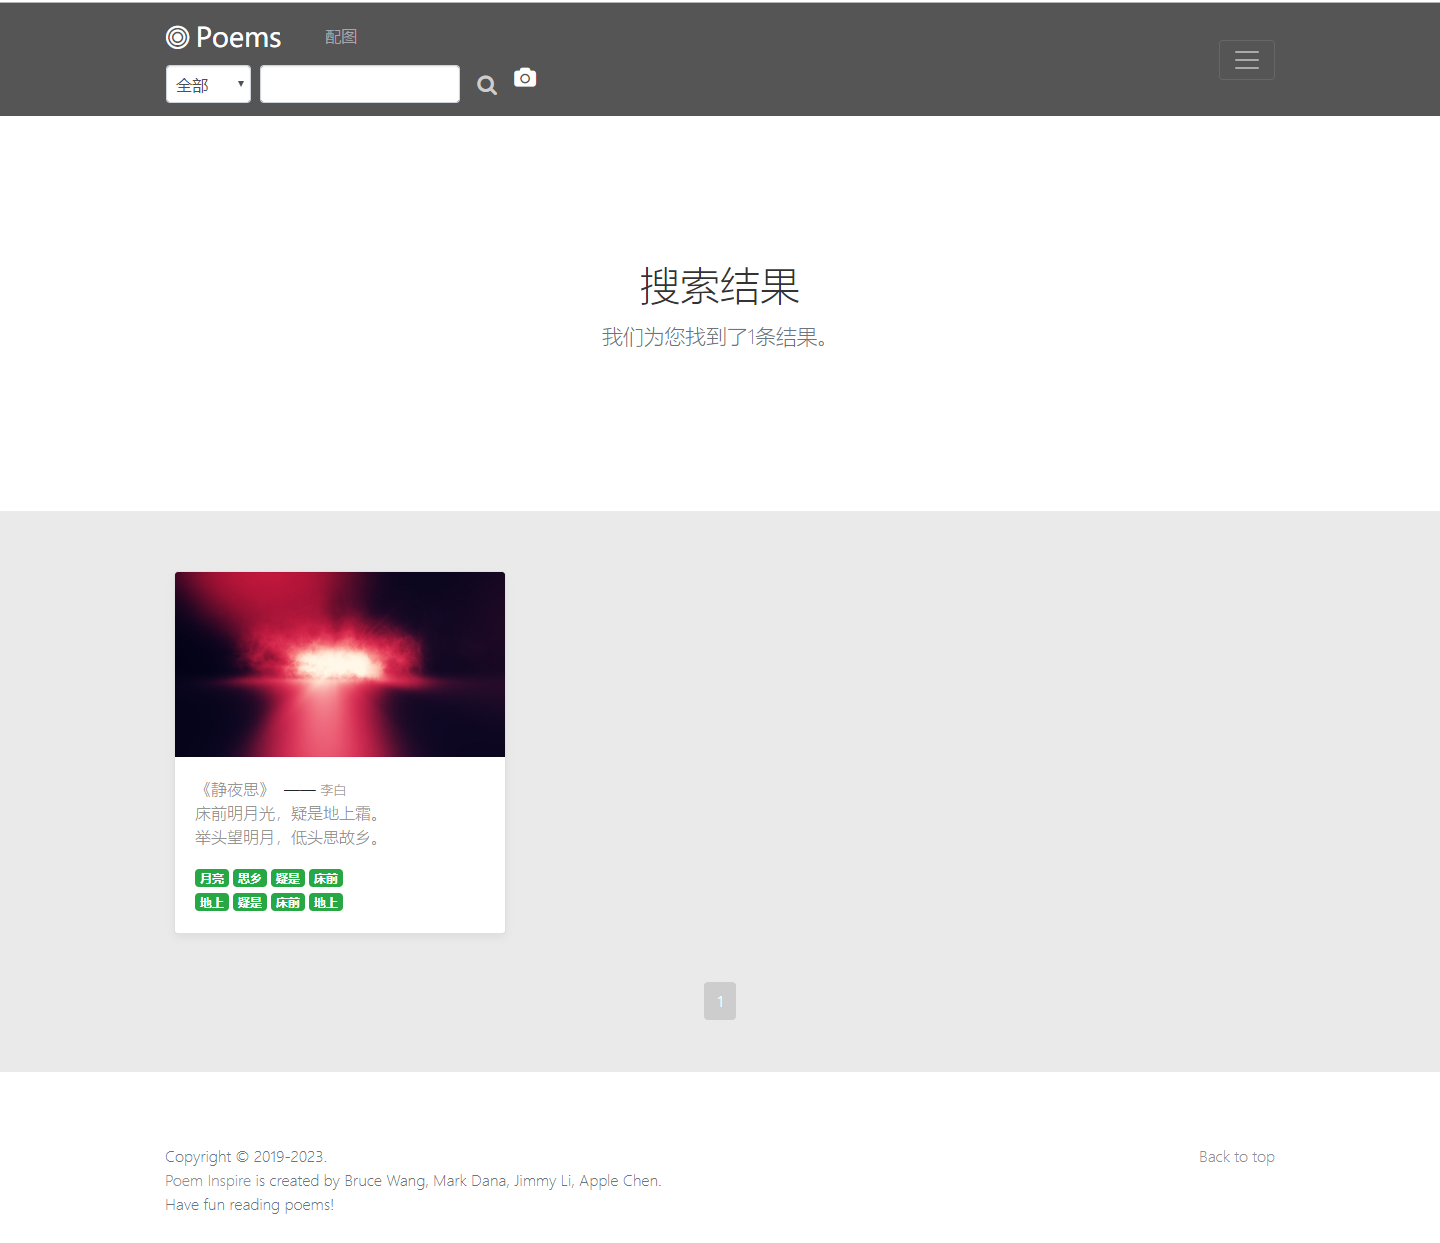
\includegraphics[scale=0.48]{fig/demo_accres.png}
\caption{精确搜索结果}
\label{fig:demo_accres}
\end{figure}

点击单首诗歌可以跳转到如图\ref{fig:demo_poempage}所示的相应的诗歌内容页面。该页面会显示诗歌的完整内容、标签以及相应配图。

\begin{figure}[H]
\centering
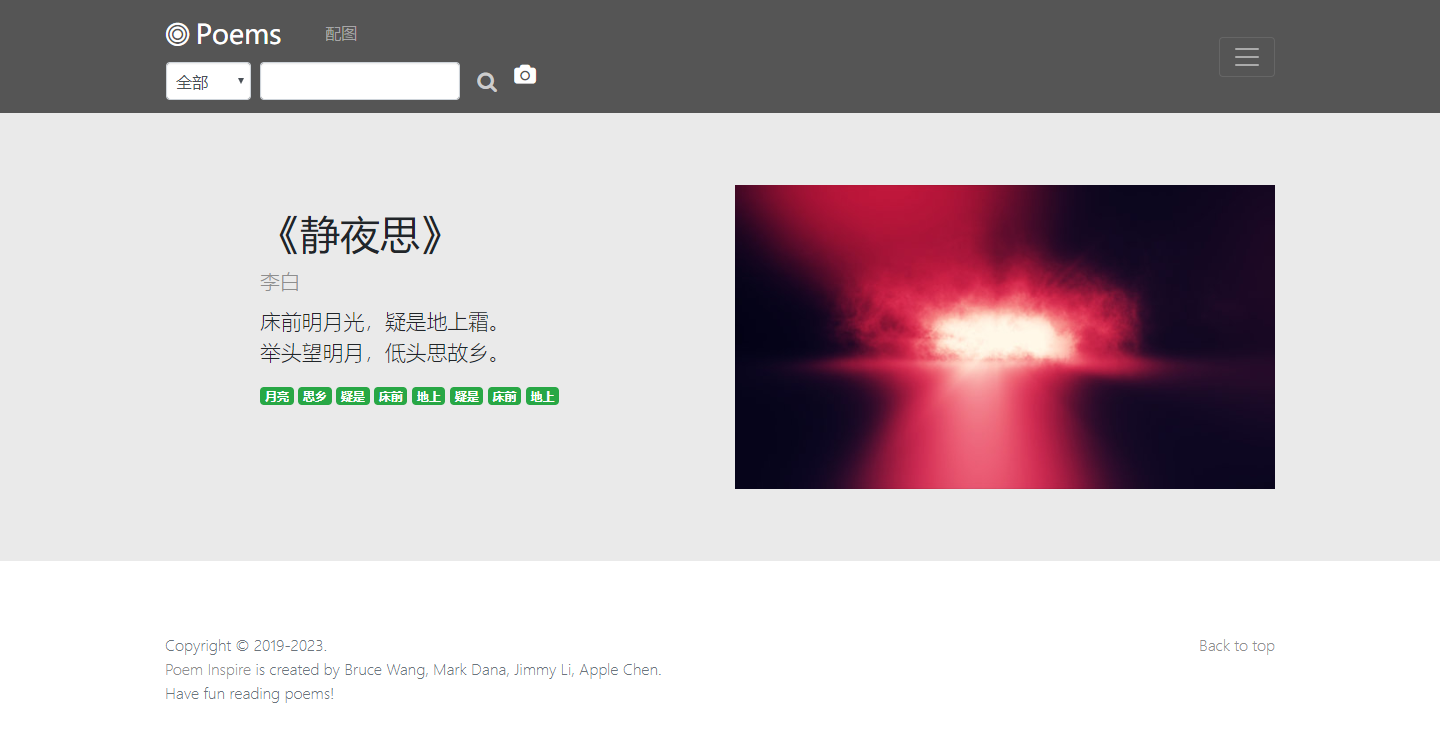
\includegraphics[scale=0.48]{fig/demo_poempage.png}
\caption{单首诗歌内容页面}
\label{fig:demo_poempage}
\end{figure}

如果解除精确搜索,并在所有域中模糊搜索“李白”这一字段,将返回如图\ref{fig:demo_vagueres}所示的结果页面。其中显示该查询共有136条匹配结果,并且每页显示一定数量的结果诗歌。

\begin{figure}[H]
\centering
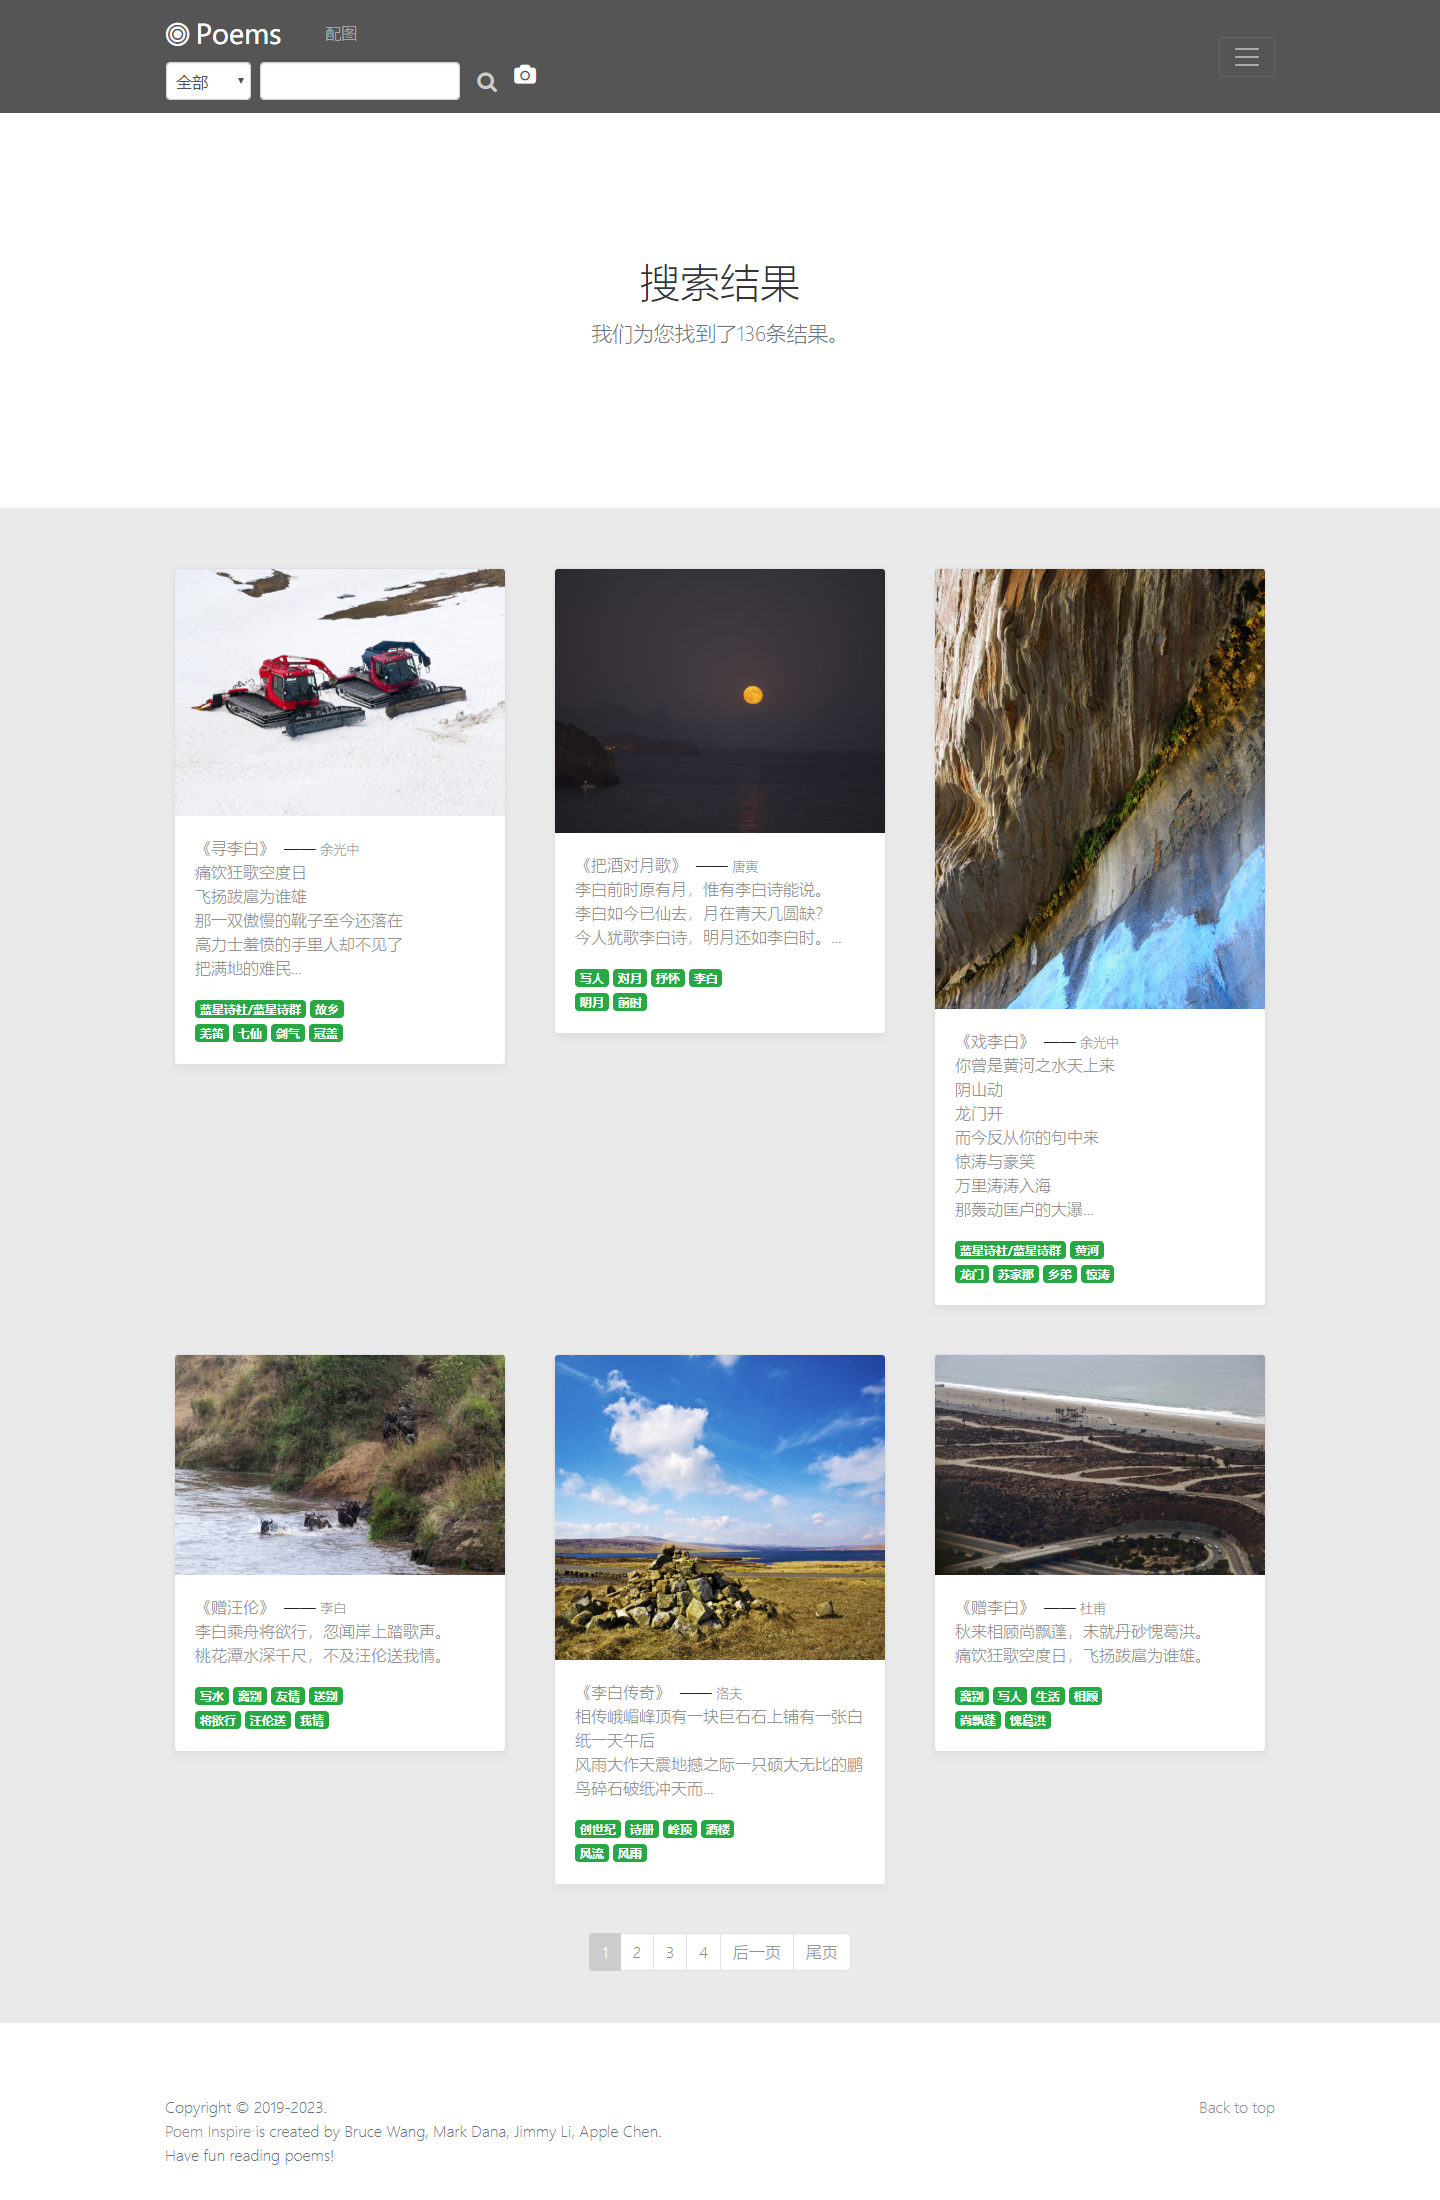
\includegraphics[scale=0.475]{fig/demo_vagueres.png}
\caption{模糊搜索结果}
\label{fig:demo_vagueres}
\end{figure}

对于每首诗歌,我们通过关键词-标签搜索为其匹配了一张图片,并通过诗歌文本分析的算法结合先前爬取的数据对其添加合适的标签,同诗歌一起展示给用户。如果诗歌长度过长,将会截断一定长度后显示。在电脑浏览器上看,每条结果的大小参差不齐,但我们是针对手机端开发的网站,在手机端上浏览效果比较好。由于结果数目较多,我们实现了搜索结果的分页显示。

用户也可以浏览单个作者的信息及其所有作品,该页面同搜索结果页面采用相同的实现形式和页面效果,再次不再作图片展示。


\paragraph*{诗图转换} 除了文本搜索,我们还实现了图片与诗歌间的转化。图\ref{fig:demo_analyze}所示为图像分析页面,这里显示了对用户上传的图片的分析结果,用户可以在分析结果的基础上进一步搜索诗歌或者生成诗歌。图中是现代诗生成结果的样例。

\begin{figure}[H]
\centering
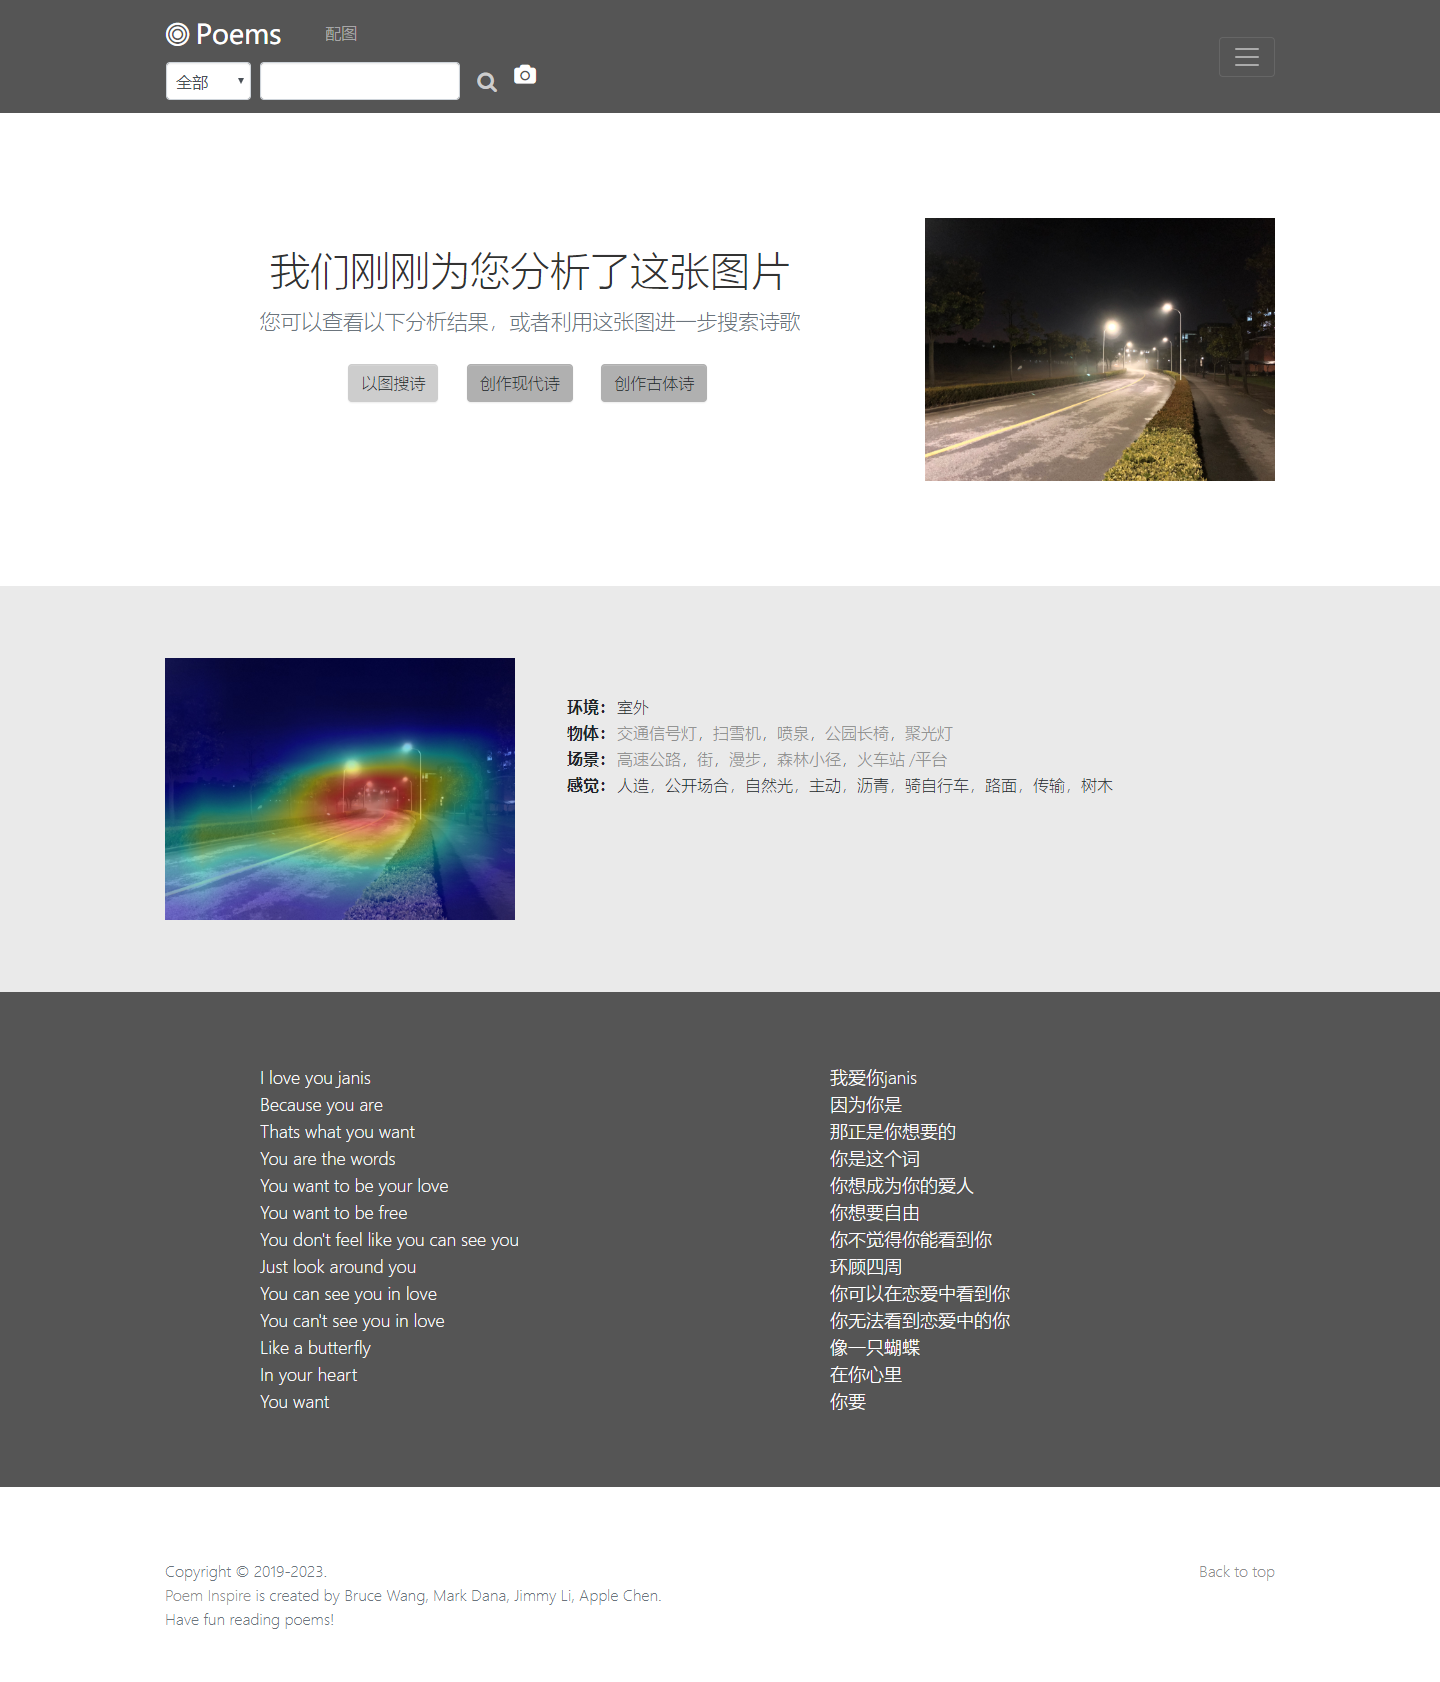
\includegraphics[scale=0.48]{fig/demo_analyze.png}
\caption{图像分析页面}
\label{fig:demo_analyze}
\end{figure}

图\ref{fig:demo_matchimage}是诗歌配图页面的样例。这里,用户可以上传自己创作的诗歌,并为这首诗歌匹配图片。图中以“青草在奔跑”为例进行配图,结果中以奔跑为主题的图片居多。

\begin{figure}[H]
\centering
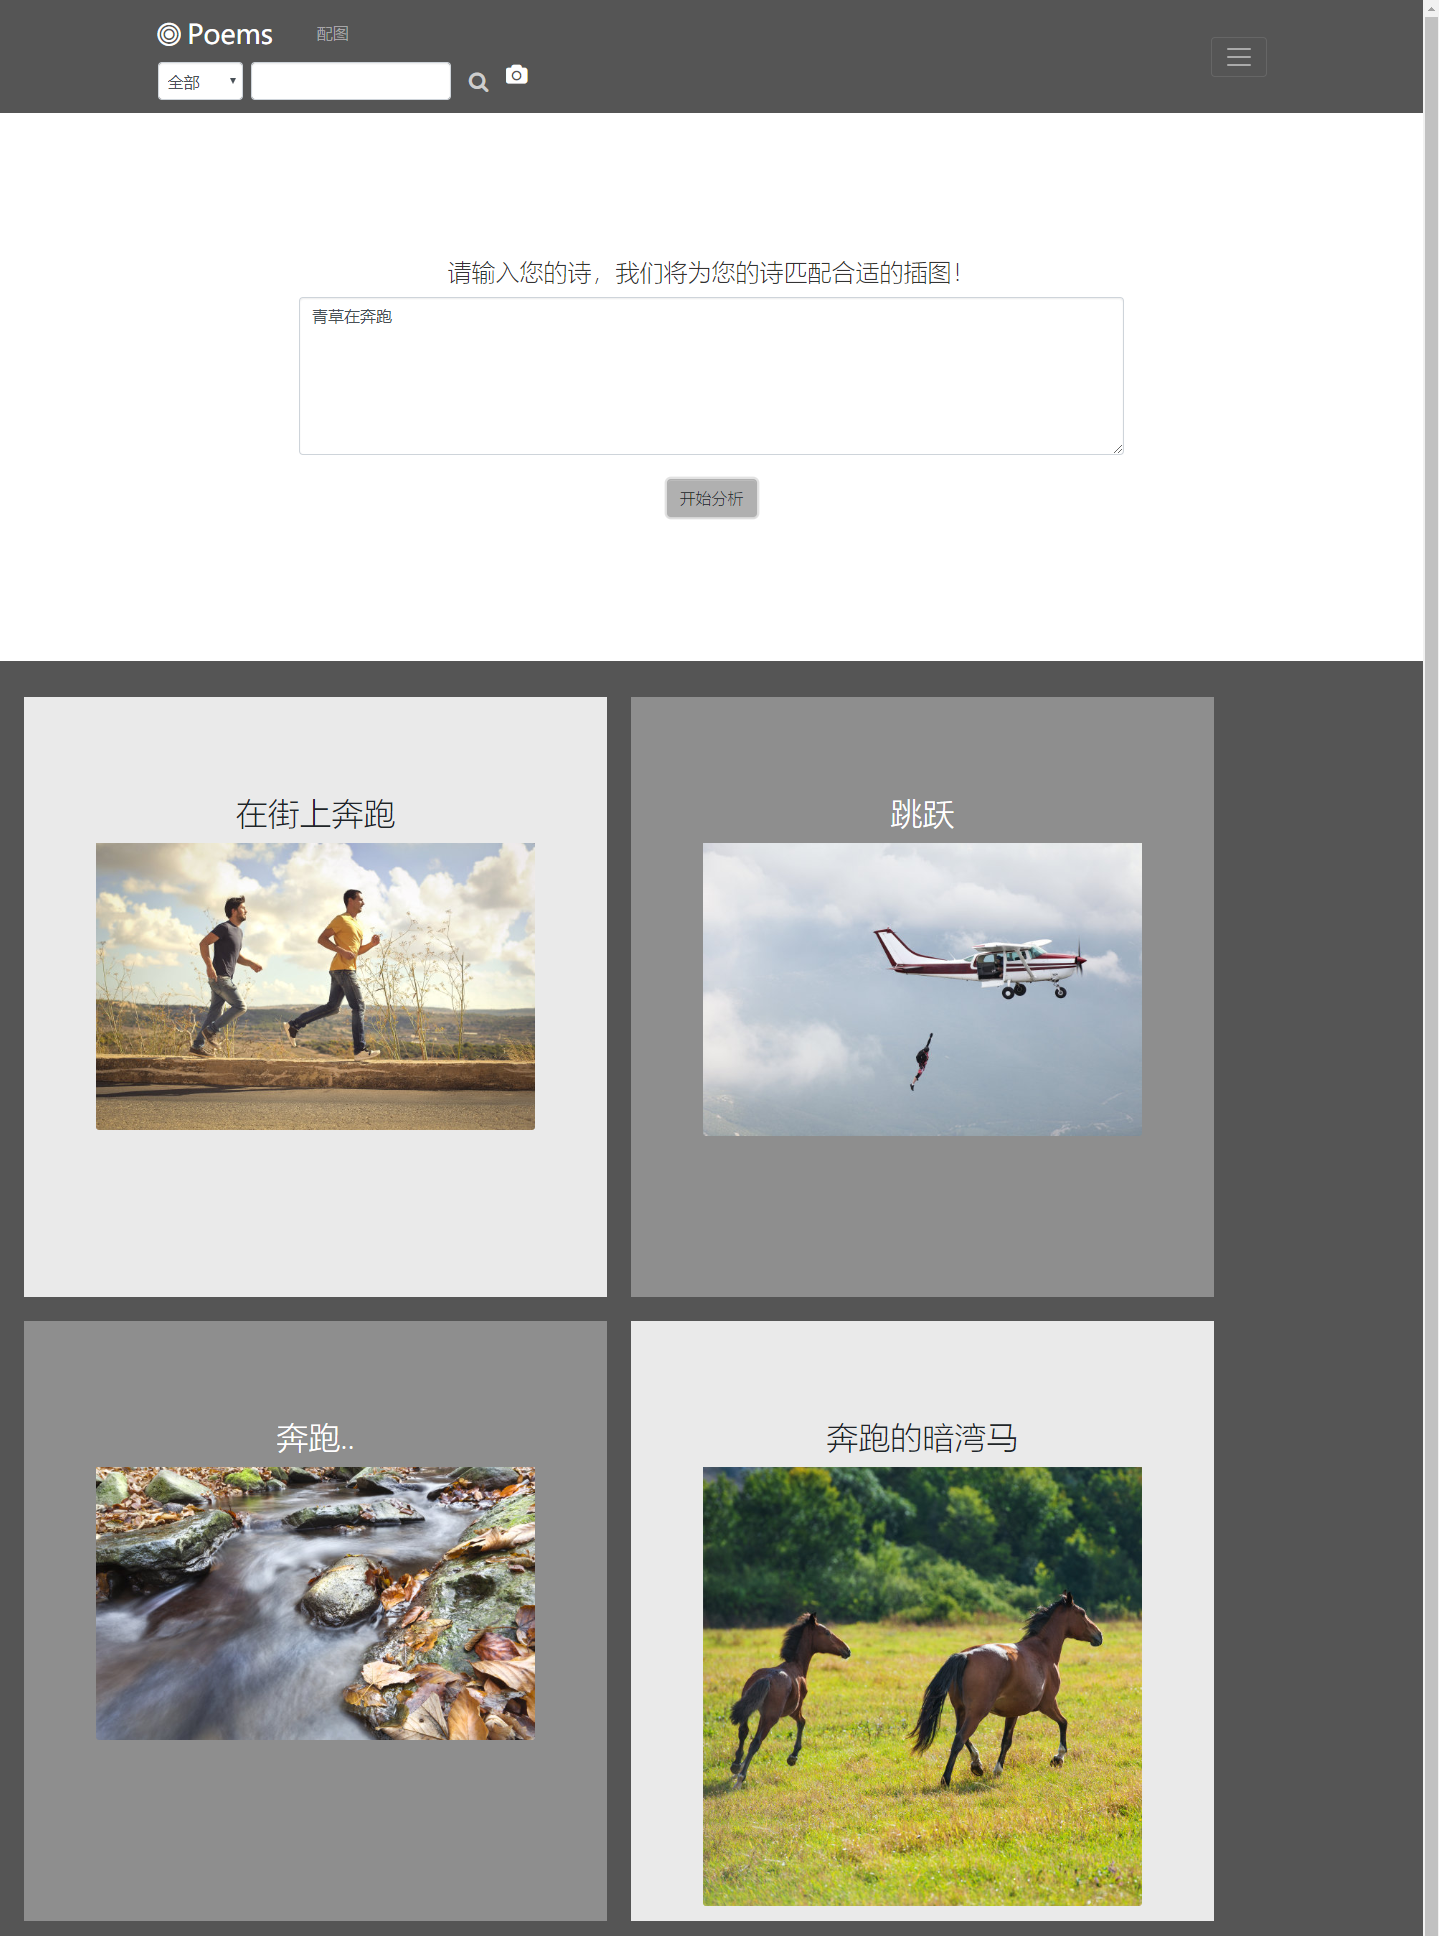
\includegraphics[scale=0.48]{fig/demo_matchimage.png}
\caption{诗歌配图页面}
\label{fig:demo_matchimage}
\end{figure}

以上便是我们搜索引擎的展示,接下来我们会详细介绍各部分的实现细节。

\section{数据爬取及处理}
项目诗歌来源包括中国诗歌网、诗歌大全文库、古诗文网等,包括现代诗与古诗这两大门类。图片来源除了上述中国诗歌网的诗影栏目,还有veer图库。

\subsection{数据爬取}
\paragraph{中国诗歌网} 该网站没有反爬虫机制,可以进行比较方便的爬取。网站目录中一页有60个现代诗的网址。注意到网站信息包含诗的ID信息体现在网站的URL中,但ID是随机跳跃的递增序列,所以我们无法直接根据URL的信息来获取所有网站。我们一开始采取的方法是先选取一个现代诗的页面作为种子,然后进入该页面根据其“下一页”的链接作为爬取的下一个网站。但这样的做法有一个很大的缺陷是爬虫的鲁棒性太低,因为一个页面最多只能生成下一个页面的链接,遇到错误时程序就会终止。最后采取的方案是,根据目录中的页数,每10页选择1个种子,并使用多线程进行爬取,每次爬取依然选择使用用“下一页”获取下一个链接放入队列,并设置每次爬取的最大页面数为5000。由于队列先进先出,我们对队列依次出队的操作可以大致保证每个初始种子所引出的页面数大致相当,这样我们一次爬取的5000个网站中便能保证其中的页面不会有重复。由于该网站数据量较大,我们对上述程序做了分布式处理,可以在多台电脑上同时爬取,提高速度。

\paragraph{古诗文网爬取}
古诗文网(https://www.gushiwen.org/)中包含了中国古代大部分的诗、词、曲、文,并提供了相应的翻译、注释、赏析、标签标注等额外信息。我们希望可以将这部分数据加入到我们的数据库中,实现较完备的搜索功能。

但是,我们发现古诗文网仅有诗歌的内容是通过静态的方式加载的,其余额外信息是通过javascript动态加载的,无法通过BeautifulSoup解析。于是,我们使用selenium模拟浏览器访问,通过模拟鼠标点击相关按钮来取回上述的额外信息。我们使用BeautifulSoup和selenium同时配合爬取,主要利用静态网页下对每首诗歌的ID的信息,来确定对应按钮的ID来实现点击。虽然使用selenium会大幅降低爬取速度,但由于该网站限制了最大页数为1000,所以总体时间还是可以接受的。

\paragraph{VEER图片数据爬取}
VEER(https://www.veer.com/)是一家免版税、国际化的微图提供商,其中提供了大量高质量的风景及其他主题的图片,我们主要使用其中的图片作为搜索引擎的图片数据。其高清图片需要付费购买才能使用,所以我们只使用了低质量的缩略图,并给出了原始VEER图片链接。

再爬取该网站的时候,我们发现Urllib和BeautifulSoup无法解析其源码,原因是该网站存在反爬虫机制,会对HTML源码注入使爬虫失效的内容。针对这种机制,我们采取了利用selenium调用javascript来强制返回其完整源码的方法。为了最大限度地降低selenium爬取时间,我们采用了先下载全部页面再解析的方式,所幸该网站可以通过URL来设定单页图片显示数量(很不明智的设计,但其后端限制了最大返回数量为200),我们通过设置显示数量为200的方式降低了selenium的调用次数,从而减少爬取时间。

我们对其中的“风光”关键字的图片进行了爬取,总计约18万张图片。


\subsection{数据处理}
\paragraph{网页信息提取}
以诗影为例,它是中国诗歌网的一个栏目,它包含了整理好的现代诗及其配图。每个页面都包含一组现代诗及其对应的一张图片,页面结尾处注明了该组诗歌的作者信息。通过分析网站结构可知,每首诗第一行为标题,其后为正文,然后接一张图片。在页面开头有作者姓名和收藏数,收藏数可作为诗影文章受欢迎程度的依据。综上,先爬取原网页,再通过BeautifulSoup提取每首现代诗的标题、作者、正文、配图地址和收藏数这些信息,并将这些信息导出为json文件,方便后续处理。古诗文网中的古诗除了上述信息,还有朝代、标签、译文、赏析等信息,均提取出来以备存。

\paragraph{多源信息整合}
现代诗的来源有多个,包括中国诗歌网的两个栏目和诗歌大全文库,将两部分来源的数据整合为统一的json,综合其标题、作者、正文、配图等信息,古诗文还需考虑朝代、诗体等。作者信息也需抽取出来单独做一个数据文件,方便后续索引。

\section{建立索引}
在此节中,我们将介绍我们为获得的数据建立索引,创建数据库的流程。

我们最初使用lucene建立索引,之后由于我们更大量数据与更深层次的搜索需求,我们放弃了lucene,而选用ElasticSearch 6.5.4作为索引和搜索的工具。

\subsection{初步索引}
使用elasticsearch建立索引,首先需要定义索引的映射,及文档中不同字段的名称和属性。这里使用了两种类型:keyword(关键词类型)和text(文本类型)。keyword指不进行分词,仅能根据精确值进行查找的字段;text指进行分词,可以由不同搜索算法进行搜索的字段。以现代诗为例,它包含了标题、作者、正文、配图等信息。配图地址采用keyword,其他采用text。作者字段可能包含多个作者,之前整合数据时进行过处理,使作者间用空格相隔,所以用whitespace分词器进行索引和搜索。标题和正文各使用两个字段,一个保存原文(如text),另一个保存进行过分词处理的原文(如text\_tokenized)。索引分词采用ik\_max\_word分词器,它对文本做最为细粒度的拆分,即穷尽所有可能的组合进行分词。搜索分词采用ik\_smart分词器,进行最为粗粒度地拆分。具体建索引时,使用bulk批量操作,提高导入索引数据的效率。

古诗文索引与现代诗索引类似,只是字段数量更多。作者信息包括姓名、简介等,索引方式与上述建立方法类似。

\subsection{更新索引}
在索引建立完成之后根据我们之前重新获取的作者信息以及生成的新标签,我们需要对原有索引进行更新。更新主要包括:现代诗作者的信息扩充(流派、年代),古现代作者的索引整合,添加诗歌标签等。

对于现代诗作者流派、年代信息的添加,我们先将所有作者添加三个空项:time\_text,time\_key,genre分别表示年代原文(e.g.“20世纪30年代”),年代关键词(e.g.“20-30”),流派(e.g.“七月派”),然后再根据我们获取的数据将json转换为字典,运用update\_by\_query()方式,对作者姓名做匹配,并添加相应信息。

对于古现代作者的整合,我们将古代、现代作者合并到一个author索引中,并新增一个字段来区分古代、现代作者。

对于添加诗歌标签,我们主要运用jieba.analyse.extract\_tags()方法。对于现代诗歌,因为其已经与我们日常用语很接近,所以我们直接用结巴的默认库,对其提取最相关联的$5$个标签。我们限定我们提取的标签为名词(“n”)以及地名(”ns”),因为这些词语一般能包含更加具体和重要的信息。对于古代诗歌,我们仍然是基于TF-IDF算法进行关键词抽取,用set\_dictionary()的方法将主词典设置为古词词典(“guci\_dict.txt”),并设置频率文件: jieba.analyse.TFIDF(idf\_path='guci\_idf.txt'),频率文件为在我们数据库里的诗歌中所有词语所出现的频率,我们运用jieba.analyse.extract\_tags()方法选取前三个匹配,并且添加到原来古诗标签字段后(原来的标签是基于诗歌的分类,比如“唐诗”、“给孩子的诗”等)。最后,我们用update\_by\_query()的方法,按诗歌ID对古诗和现代诗分别添加和修改标签项。

\subsection{给诗配图}
我们首先确定了基于关键词-标签搜索的诗图互搜算法,算法原理如图\ref{fig:poemimg}所示。
\begin{enumerate}[(1)]
    \item 由诗搜图的过程是由诗的关键词进行同义词扩展后搜索图片的联想词。若由诗的全文分词进行搜索,则查询信息数据量较大,且缺乏有效信息。而关键词通过结巴的tf-idf算法进行抽取,其本身是文章重要信息的提炼,查询有效性提高。
    \item 由图搜诗是由图的联想词搜索诗歌的全文。图片的联想词已经进行过同义词古词扩展,搜索全文(分词后的)可以匹配更多的信息,对古诗文部分也有所兼容。
\end{enumerate}

根据上述诗图互搜的两种方式,诗配图也有两种方案。
\begin{itemize}
    \item 方案一:遍历诗歌,通过诗歌查询图片,将评价最高的图片作为其匹配图。
    \item 方案二:遍历图片,通过图片查询诗歌,在评价得分最靠前的五首诗中,选择未配图的第一首诗作为该图的对应。
\end{itemize}

数据库中图片有18万张,而诗歌数只有3万。经过测试,第一种方案速度约为1秒5首诗,第二种约为3秒一张图,所以第一种方案速度更快。两种方案均存在诗歌未匹配上图片的情况,后一方案以图片为主体的搜索使这一情况更容易发生,因此还需采用前者对剩余诗歌进行配图,增加了工作量。综合考虑,我们采用了第一种方案。
\begin{figure}[H]
\centering
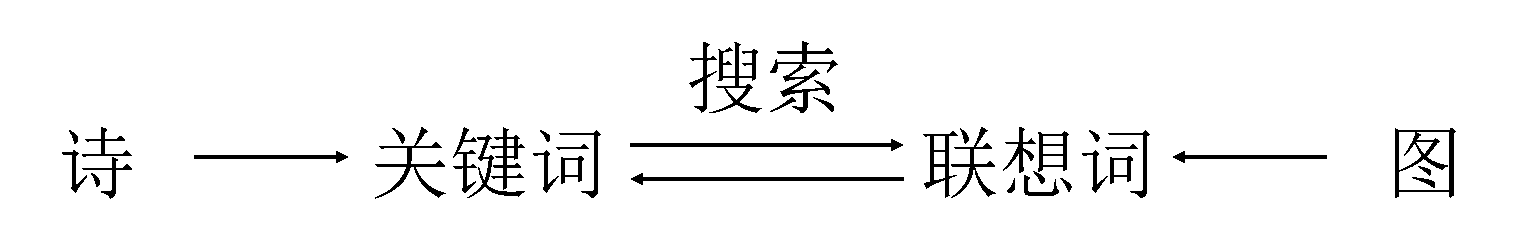
\includegraphics[width=0.8\linewidth]{fig/poemimg.png}
\caption{诗图互搜算法原理图}
\label{fig:poemimg}
\end{figure}


\section{后端实现}
在这一部分,我们将介绍搜索引擎的后端实现,包括网站的后端实现和数据库搜索的实现。

\subsection{网站架构}
图\ref{fig:web_struct}是我们搜索引擎的网站架构。

\begin{figure}[H]
\centering
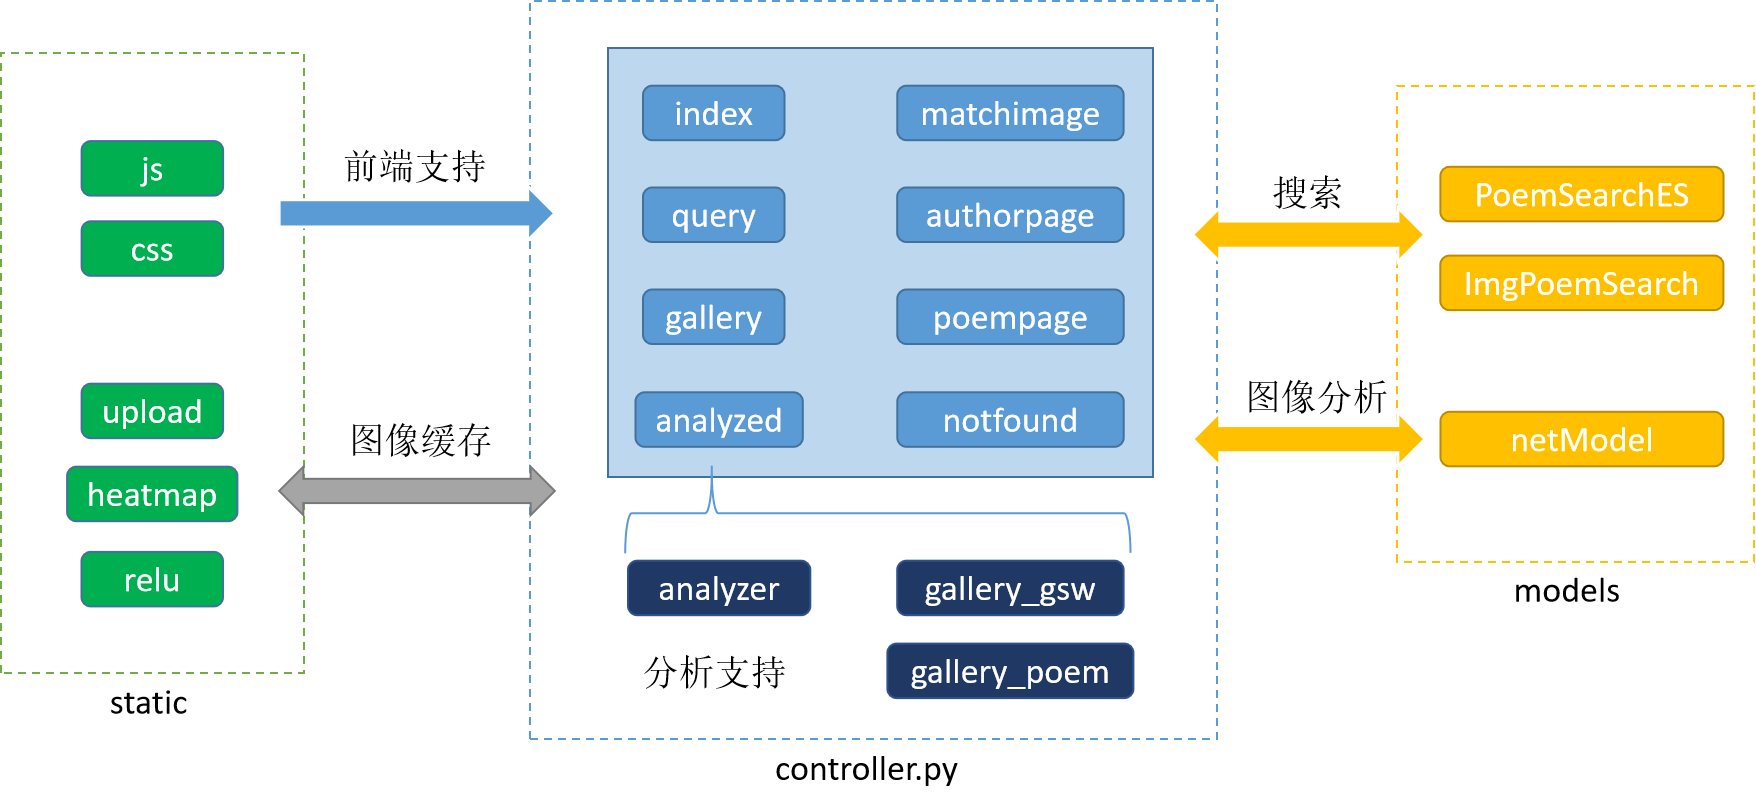
\includegraphics[scale=0.48]{fig/web_struct.png}
\caption{网站架构}
\label{fig:web_struct}
\end{figure}

我们的网站采用了一定的MVC分离。PoemSeachES和netModel及model文件夹下的模型为搜索引擎的模型部分,负责对controller发出的查询请求做出响应和进行图像处理。controller.py为我们的控制器,图中由淡蓝色矩形框出的类都有对应的前端页面,深蓝色标出的三个类通过前端的javascript进行动态加载,异步返回数据。static是web.py框架下网站的资源文件夹,其中的js文件夹和css文件夹包含了支持前端布局的js文件和css文件,其余三个文件夹用于缓存用户上传和图像处理中间结果的图片。

\begin{table}[H]
\centering
\begin{tabular}{ccc}
\hline
\textbf{类} & \textbf{URL} & \textbf{页面} \\ \hline
index & /index & 首页推荐 \\
query & /query & 文本和图像查询处理结果页面,无翻页功能 \\ 
gallery & /gallery & 同query,但只处理文本查询,提供翻页接口 \\ 
poempage & /poempage & 单首诗歌内容页面 \\ 
authorpage & /authorpage & 单个作者信息及作品页面,类似gallery \\ 
matchimage & /matchimage & 诗歌配图页面 \\ 
analyzed & /analyzed & 图像分析页面 \\ 
notfound & /notfound & 404页面 \\ \hline
\end{tabular}
\caption{链接对应关系}
\label{tab:url_connect}
\end{table}

controller中各个类对应的url及前端页面功能如表\ref{tab:url_connect}所示。

在controller.py中,我们还有一系列辅助函数存放在validator类下,用来进行表单验证和表格输入的预处理。其中最主要的两个函数是form\_validate和to\_command\_dict。

form\_validate对于用户通过表单的输入进行验证并返回验证结果供调用者进一步判断页面的跳转。该函数会判断用户的输入是否为空,其会检查所有可能成为有效输入的域,包括高级搜索中的精确搜索域。该函数还会检查表单输入的合法性,来避免用户的恶意访问。两个关键的准则是表单中包含searchType和query这两个域,因为他们确定了查询的索引和查询的内容(虽然query可以为空),和存在query模糊查询时高级搜索中的搜索域选择非空,否则这条查询无法转化成模型可以处理的命令。对于其他只应该由我们规定的内链所引起的查询,我们或者重用了form\_validate,或者实现了各自的验证函数来保证没有会造成严重后果的恶意访问发生。

to\_command\_dict根据表单提供的不同的查询约束,生成对应的查询域和查询值的映射并规定每一条约束是否为强制的(精确查询的)。这个函数的意义在于实现搜索引擎建立与数据库建立、控制器与模型的解耦,避免了在多个文件中修改关键字名称的工作。

\subsection{索引搜索}

在我们的索引搜索中,图片搜索是前文给诗配图这一功能的复用,在此节中不多加赘述,我们将着重介绍我们是如何利用elastic-search实现基于文本的诗歌搜索的。

\paragraph*{布尔查询} 我们充分利用了elastic-search的布尔查询的灵活性,从而得以实现复杂的符合查询。从控制器中传入到后端搜索模型的数据都是经过处理的命令字典,其中每个条目的关键字已转换成数据库中的搜索域的关键字,每个条目的值是一个包含查询内容和是否使用了精确查询的布尔值,该字典形如$\{ \text{[关键字]}: (\text{[查询内容], [是否精确查询]}) \}$。

对应古诗文的关键字有:“author”(作者),“dynasty”(朝代),“label\_tokenized”(标签), 
“title\_tokenized”(标题),“text\_tokenized”(诗歌正文),“shangxi\_tokenized”(诗歌赏析), “yiwen\_tokenized”(诗歌翻译)。

对应现代诗的关键字有:“author”(作者),“title\_tokenized”(标题),“label\_tokenized”(标签),“text\_tokenized”(诗歌正文),“genre\_key”(流派),“time\_key”(年代)。

对于每条查询,我们都准备了一个包含should(选择性出现)和must(必须出现)两个列表的字典作为搜索主体,对于命令字典中的合法条目添加到对应的列表中。如果使用了精确查询则将子查询体加入到must列表,否则加入到should列表。在常规情况下,我们使用match\_phrase作为查询方式,这种情况下,进过elastic分词分析后的每个词组必须按顺序完整地匹配上对应域中的一段子字符串才算是一次命中。如果搜索是由同义词扩展、或者图片搜诗发起的,则使用条件较宽松的match方式进行查询。

在查询的时候,我们首先利用elastic的count查询取回总共的匹配数量,再通过函数调用者规定的结果页数、每页显示数量等确定取回的记录在所有排序后的匹配中的区间,利用search方法取回搜索结果。

\paragraph*{搜索结果后处理} 搜索结果是以elastic的json放回格式构造的,不便于控制器和前端显示使用,因而我们在返回结果前调用process\_query\_results函数对搜索结果列表进行格式化处理。该函数会对诗歌显示长度进行调整,对每条结果的字典关键字进行重命名,配置内链的URL,对其他的显示内容进行适当的调整等。如此一来,我们实现了MVC三者较高程度的解耦,方便后续功能的扩展和调整。其他类型的搜索也采用了类似的方法进行后处理,后续将不再对此赘述。

上述类型的布尔查询主要用在对于诗歌的查询上,这也是我们搜索引擎最主要的查询功能。我们有cnmodern\_search(现代诗查询)和gushiwen\_search(古诗文查询)两个主要的查询函数,采用上述实现方式。对于mixed\_search(混合查询),我们采用每次取回各占显示数量一半的现代诗和古诗文策略,复用以实现的单类型查询函数。这样做唯一的不足在于如果缺少某一种类型的搜索结果,前端只能显示一半数量的结果。但这样做却能保证我们的分页查询正常工作。

\paragraph*{分页查询} 我们的分页采用from-size的深度分页,及每次查询取回一定排序区间内的结果,这需要反复取回同一段结果并进行排序,效率较低。而且,elastic对于from-size查询方式的查询上限有一定限制,每次最多只能取回10000条结果,我们将这一上限扩大到50000来应对较大的查询量。这并不能从根本上解决问题,我们可以利用elastic的scroll查询方式来实现高效的分页查询,但由于时间问题,我们只能止步于目前的深度分页模式。

\paragraph*{作者查询} 作者查询并不是我们搜索引擎的核心查询,但也是其中必不可少的一部分,因为我们需要对一个作者的作品进行展示并允许用户通过一首诗了解其作者的其他作品。搜索作者时,我们采用了使用match\_phrase命令来匹配作者姓名来搜索结果。但稍后我们发现可以使用elastic数据库的内置ID来准确的取回某个作者的结果,现在的方法对于重名作者将无能为力。由于时间问题,我们未能及时改善此处的查询。get\_author\_poems函数实现了作者诗歌的分页查询,get\_author\_desc用于取回单个作者的简介。

除了上述查询,我们模型部分还有基于elastic数据库内置ID的单首诗歌的取回和推荐取回,这部分的查询实现较为简略,在此不多加赘述。


\section{图片-诗歌生成模型}
整个图片生成诗歌的步骤可分为三步:图像特征提取、特征词义扩展和诗歌生成。

\subsection{图像特征提取}
对传入图片进行卷积神经网络运算,得到多分类预测,包括图片的物体、场景和情态特征。在电工导课堂上我们学习图像处理中的如sift算子、sobel算子等,也可以理解为单层的卷积操作。

我们使用了\href{http://www.cs.toronto.edu/~frossard/post/vgg16/}{基于ImageNet训练的vgg16结构}来预测图片的object特征。直接由最后一个全连接层的softmax输出得到对1000分类的object信息预测。

而对于图片的scene和emotion信息,我们使用了\href{http://places2.csail.mit.edu/PAMI_places.pdf}{基于Places365训练的ResNet18结构}来预测。其中scene信息来自原模型365维的输出,根据原标签事先对室内外的区分,也可以得到平均的室内外判断。利用pyTorch的hook功能,我们钩取了全连接层前的平均池化层的输出,一个512维向量;原网络提供了102*512维关联矩阵,表征avgpool层输出在102个动作情态特征上的关联度、判据,将该关联矩阵和512维向量点乘,就可以得到标签的贡献特征,这些attribute特征具有情态性,我们用它来反映原图的emotion特征。

\begin{figure}[H]
\centering
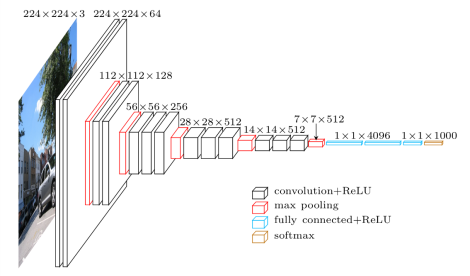
\includegraphics[width=0.6\linewidth]{imgs/1.png}
\caption{vgg16网络结构}
\end{figure}
\begin{figure}[H]
\centering
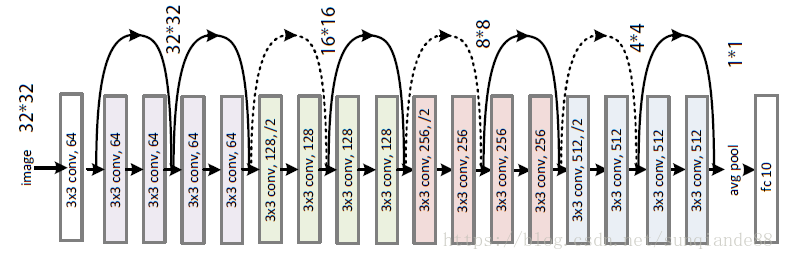
\includegraphics[width=0.6\linewidth]{imgs/2.png}
\caption{resNet18网络结构}
\end{figure}

同时,为了增强该cnn网络的可解释性,还钩取了layer4层,也就是最后一个卷积层在残差层之后的输出,一个$512\times 14\times 14$维矩阵,将该矩阵与最后softmax层的权重向量点乘,即是最终权重与该conv层的综合触发,分析得到结果矩阵中的每个点的邻域,得到其featuremap,寻找局部极大值,就认为这是触发峰,也就是原图中相应位置的某些特征对预测结果有较大贡献。然后将该结果矩阵以热力图的方式覆盖,用户就可以看到原图各区域对结果的触发程度。

\begin{figure}[H]
\centering
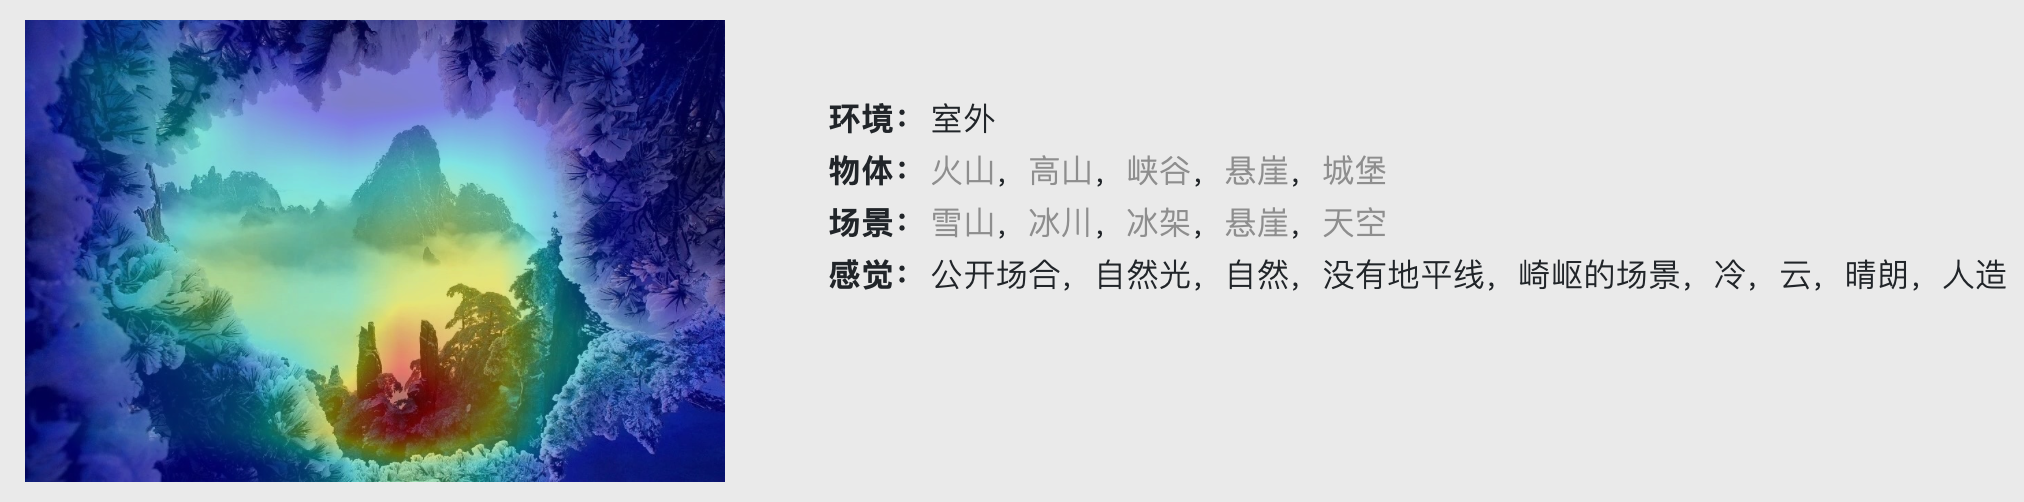
\includegraphics[width=0.8\linewidth]{imgs/3.png}
\caption{图像特征抽取展示}
\end{figure}

\subsection{特征词义拓展}
通过上一步骤的cnn我们已经得到了图片的特征信息,但输出的特征最终需要用语言来展示。原数据集(ImageNet和Places365)中的标签均是英文,直接翻译成中文也是现代汉语,比如——
\begin{framed}
物体:山雀,石榴,CD播放器,巧克力酱...\\
场景:轿车轿厢内、湖泊、山间小路、海滩...\\
感觉:清洁的,日光浴、崎岖的、遥远的...
\end{framed}

这些词语直接翻译是现代汉语,并且具有西式生活色彩。直接以这些词语去搜索或生成古诗显然是愚蠢的,我们没法期望在古诗里搜到‘轿车轿厢内’,也当然不能生成一首古诗,开头是‘CD播放器’。那么如何填补古汉语与现代汉语之间的差异,建立词义拓展的联系呢?

\subsubsection*{word2vec学习}
初始时我们尝试了用word2vec方法来做近义词拓展。可以理解为用某个长度的滑窗对文本进行卷积,在原文本中位置相距越近的词,我们认为词义上的关联就越大。而每个词用某长度的向量来表示,词义间的关系则通过向量间余弦表示。但是仔细思考后发现这个方法并不可行,因为第一,在这种近义词任务中,简单地以距离作为相似度判据并不可靠,距离只能代表关联性,比如“我”“爱”“你”,“我”和“爱”在文本中关联性较大,但不是近义词。第二,也是最主要的原因,我们很难获取到包含古文和现代词的文段,而直接对所有古诗进行seq2seq学习,也只能得到古文间的词义聚类,并不能和现代汉语产生关联。因此我们考虑另外的方法。

\subsubsection*{古词库与现代汉语近义词库}
随着继续探究问题,我们发现了两个对解决问题有关键作用的数据库。第一个是《诗学含英》,是清代刘文蔚根据《增广诗韵全璧》一书所附〈诗学含英〉创作的一本工具书,包含了9000余古诗中出现的意象、词语,按照天文、时令、节序、地舆..等分类;另一个数据库是哈工大的《同义词词林》,词林的格式是6级编码,其中前五个是类别级别,大中小类、词群和原子词群,而第6位编码是标记位,注明词语关系。如:
\begin{framed}
Aa01A02= 人类 生人 全人类
\end{framed}

利用对每个级别分配权重并将词义间关联用编码的向量余弦角表示的方法,可以求得现代汉语之间的词义相似度。这个功能在Python中有封装好的第三方库`synonym`,我们直接调用了。如果用图的观点来理解,我们已经有了一个边较稠密的现代汉语森林,和一个边较稀疏的古词森林,如何将这两个森林建立联系呢?

\subsubsection*{利用翻译}
我们考虑对于《诗学含英》中的每一个古词,利用在线翻译将其翻译为英语,借助英语这个中介,再翻译回汉语,就可得到相应的现代文近同义词;再利用同义词林的方法,获得该现代词的前k个同义词(按照相关度即余弦角排序),这样这$k+1$个现代汉语词就都和该古词建立了对应关系,对应的关联程度按照相关度来定义。遍历所有古词之后,大部分现代汉语就都有了其对应的一群近义古词和相应的相关度。完整的流程比如:

蜜尤香$\rightarrow$Honey$\rightarrow$蜜糖,蜂蜜$\rightarrow$蜂蜜,牛奶,汁,糖浆,果汁,葡萄,水果,马铃薯,肉桂, 杏仁$(1.0,0.72741085, 0.72632432, 0.71830636, 0.71781552...)$

最终“巧克力酱“、“奶酪软饼“、“馅饼“、“糖酥派“等现代词语都可以联想到古词“蜜尤香”。回到上面展示的几个现代词,联想如下(按照相关度排序):

% Table generated by Excel2LaTeX from sheet 'Sheet1'
\begin{table}[H]
  \centering
  \caption{现代词-古词联想}
    \begin{tabular}{|l|l|}
    \hline
    现代汉语  & 古词 \\
    \hline
    山雀    & 山鸟,啄木,鹭鸥,鹭,鸳鹭,鸥鹭,栖鹭,鹭鹚… \\
    \hline
    CD播放器 & 为盘,声频,佛阁,拖荇带,书带,碧筒,兰缸,仙机... \\
    \hline
    轿车轿厢内 & 翔车,车盖,车似,车驻,车咸,万车,车前,盈车,野马,凤胎... \\
    \hline
    山间小路  & 云壑,谷,万壑寒,春山,四隅,阡陌,客路长,林霭,幽径... \\
    \hline
    清洁的   & 洁身,轻清,清游,淡净,致洁,似冰清,心与洁,楚楚... \\
    \hline
    崎岖的   & 崎岖,峻岭,峭壁,险峻,亘地蟠,浪未平,奔崖,景难... \\
    \hline
    \end{tabular}%
  \label{tab:addlabel}%
\end{table}%


使用翻译的方法虽然简单粗暴,但是确实很有用,大多数的现代汉语词最终都匹配到了10个以上的古代同义词,建成了一个哈希散列表直接封装可搜索。这在后续的生成古诗词过程中有用;并且也可以作为一个单独的古今近同义词数据集以便后续研究。我们也参考了\href{https://arxiv.org/abs/1806.06349}{Incorporating Chinese Characters of Words for Lexical Sememe Prediction}这篇论文中建立词义关联的部分。

有趣的是,在爬取翻译的过程中,刚开始我们写的爬取谷歌翻译,由于谷歌翻译的结果并没有直接显示在网页中,而是异步返回的,我们仔细研究写了一个专用的抓包爬虫程序。然而在爬了1000多个词之后,那个程序就坏了,得换另外的ip地址——因为被谷歌的反爬虫机制识别了,对ip进行了封禁。因此最终我们使用了搜狗的翻译api接口,使用付费服务。

\subsubsection*{词频分析与提取关键词}
目前我们有了《诗学含英》这一庞大的古词数据集,也将古词森林和现代词森林之间建立了意义关联,那么接下来就可以进行词义互联等工作,用于古诗词的分词程序也有了自己的热词库,从而可以提高分词准确率。接下来我们还想对所有古诗词进行词频统计和关键词提取,获得词义间更紧密的联系,用于标签推荐等。

关键词抽取我们使用了课上学习过的TF-IDF算法,也就是Term Frequency*Inverse Document Frequency来表征某词语在全文中的关键程度。

$\displaystyle \mathrm{TF}_{i,j}=\frac{n_{i,j}}{\sum_k{n_{i,k}}}$,其中TF$(i,j)$为关键词$j$在文档$i$中的出现频率,$n(i,j)$为关键词$j$在文档$i$中出现的次数。

$\displaystyle \mathrm{IDF}_i=\log\frac{|D|}{|j:t_i∈d_j|+1}$,其中IDF$(i)$是词语$i$的反文档频率,$|D|$是语料库中的文件总数,而$|j:t(i)\in d(j)|$是出现词语i的文档总数。

同时我们也参考了TextRank算法进行关键词抽取,不需要事先学习训练,简便高效。课上我们学过PageRank算法,TextRank算法正是基于PageRank,将文段按照句子分割并分词和词性标注后,将候选关键词建模成有向有权图,想象一个滑窗(共现窗口)对文段进行卷积运算,A和B的联系,可以定义为从图中点A指向点B的概率(权重),从PageRank的角度理解,就是在A中搜到B的概率,那么按照同样的方法,将该有向图的构造边定义为:两个节点之间存在边仅当它们对应的词汇在长度为K的窗口中共现。

用$\displaystyle \mathrm{WS}(V_i)=(1-d)+d*\sum_{V_j∈In(V_i)}\frac{w_{ji}}{\sum_{V_k∈Out(V_j)}w_{jk}}WS$(其中In(Vi)为指向Vi的点集合, Out$(Vi)$为Vi指向的点集合)定义某点$V_i$的得分,在上一步骤构造的图中,迭代权重直至收敛,选出最重要的$T$个词,就是得到的该文段的$T$个关键词。

\subsection{古诗文生成}
\subsubsection*{数据预处理}
考虑到诗(尤其是绝句、律诗等)在形式、断句上较为规整,我们本次实验中只采用诗来训练网络。使用了唐诗和宋诗一共30余万首诗,初步对长度($>14$个汉字,$<200$个汉字)进行筛选、对生僻字(不在9000余字库中)、乱码等进行数据漂洗,然后对每首诗加上开始和结束标识符。这是形式上的统一。

接下来是字符映射,对每个字进行字频统计后得到其id,建立字符和id之间的映射。需要注意,对于标点符号同样要赋值id,因为在接下来的学习中没有过多的人工干预,希望模型能自己学出断句规律。另外,由于诗歌长度不同,需要填补空格id。对于每首诗构建其poem vector,即所有字(和空格凑成该batch中最长诗长度)的id组成,投入接下来的网络中进行训练。

\subsubsection*{LSTM训练}
首先划分训练集和测试集,trainRatio=0.8,即每次迭代内$80\%$的数据用于训练,$20\%$用于测试。然后构建训练batch,每个batch由64首诗构成。LSTM在文本生成等NLP任务中使用十分广泛,本质可以联系到概率论中的hmm模型等,但每个接下来单元的概率不仅与前n个有关,而是与整个前文有关,并设置了dropout层进行遗忘或增加信息等。具体原理此处不赘述。

\begin{figure}[H]
\centering
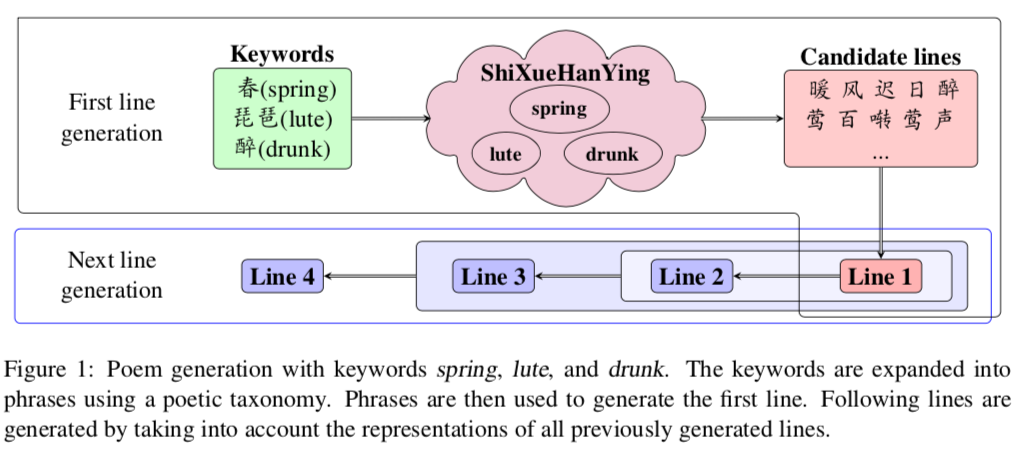
\includegraphics[width=0.8\linewidth]{imgs/4.png}
\caption{参考论文中使用的Keyword Expansion}
\end{figure}
\begin{figure}[H]
\centering
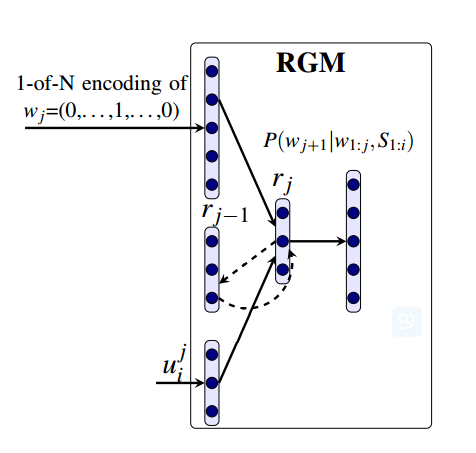
\includegraphics[width=0.4\linewidth]{imgs/5.png}
\caption{参考论文中使用的Recurrent Generation Model}
\end{figure}

我们参考了2014年发表在EMNLP上的论文\href{http://aclweb.org/anthology/D/D14/D14-1074.pdf}{Chinese Poetry Generation with Recurrent Neural Network},并最终使用了基础的LSTM模型,在TensorFlow模板上进行修改,后接一个softmax输出接下来某字的出现概率。设置2个循环隐藏层,隐藏细胞hidden\_units=128。设置学习率为0.001,并使用了TensorFlow中的衰减策略,设learningRateDecayStep = 1000,learningRateDecayRate = 0.95。损失函数设计为预测字符和语料中实际字符的交叉熵。

训练环境:Ubuntu18.04, TensorFlow1.12.0, CUDA9;四路GeForce GTX 1080Ti。总共对30万首诗训练50个epoch,共耗时约三天。

训练结果:Error Function从开始的1.9降至0.1左右。(忘了保存训练曲线..)

\subsubsection*{诗歌生成}
由某个关键字开头后,接下来每个字得到的概率向量来自之前的已有全部文段。对概率向量进行直方图统计操作,并按照概率权重随机取字,直至生成结束符,即可生成一首诗。LSTM网络可以直接生成整首诗,但为了让生成诗更加具有用户可控性,控制整体诗歌的氛围特征,我们允许用户自行加入古词关键词在各个句子中引导生成。古诗关键词的加入来自上一部分的词义联想扩展功能。

同时,我们发现该LSTM网络生成的诗歌在押韵平仄等音韵特征方面不够好,我们对生成的softmax预测概率加入了音韵惩罚。我们获取了汉字的拼音数据集,并对于生成诗歌的某些特定部位(如一三五不论、二四六分明的句尾、奇数关节)的汉字与前文的韵母和平仄进行比对,如果不符合正确的押韵及平仄规则,softmax概率乘以一个小于1的惩罚权重。另外,考虑到目前还学不到如“凄凄惨惨戚戚”的程度,生成的叠词往往造成无意义病句,我们也加入了叠词惩罚。

\begin{figure}[H]
\centering

\includegraphics[width=0.9\linewidth]{imgs/6.png}
\caption{从交大庙门生成诗歌}
\end{figure}
\begin{figure}[H]
\centering
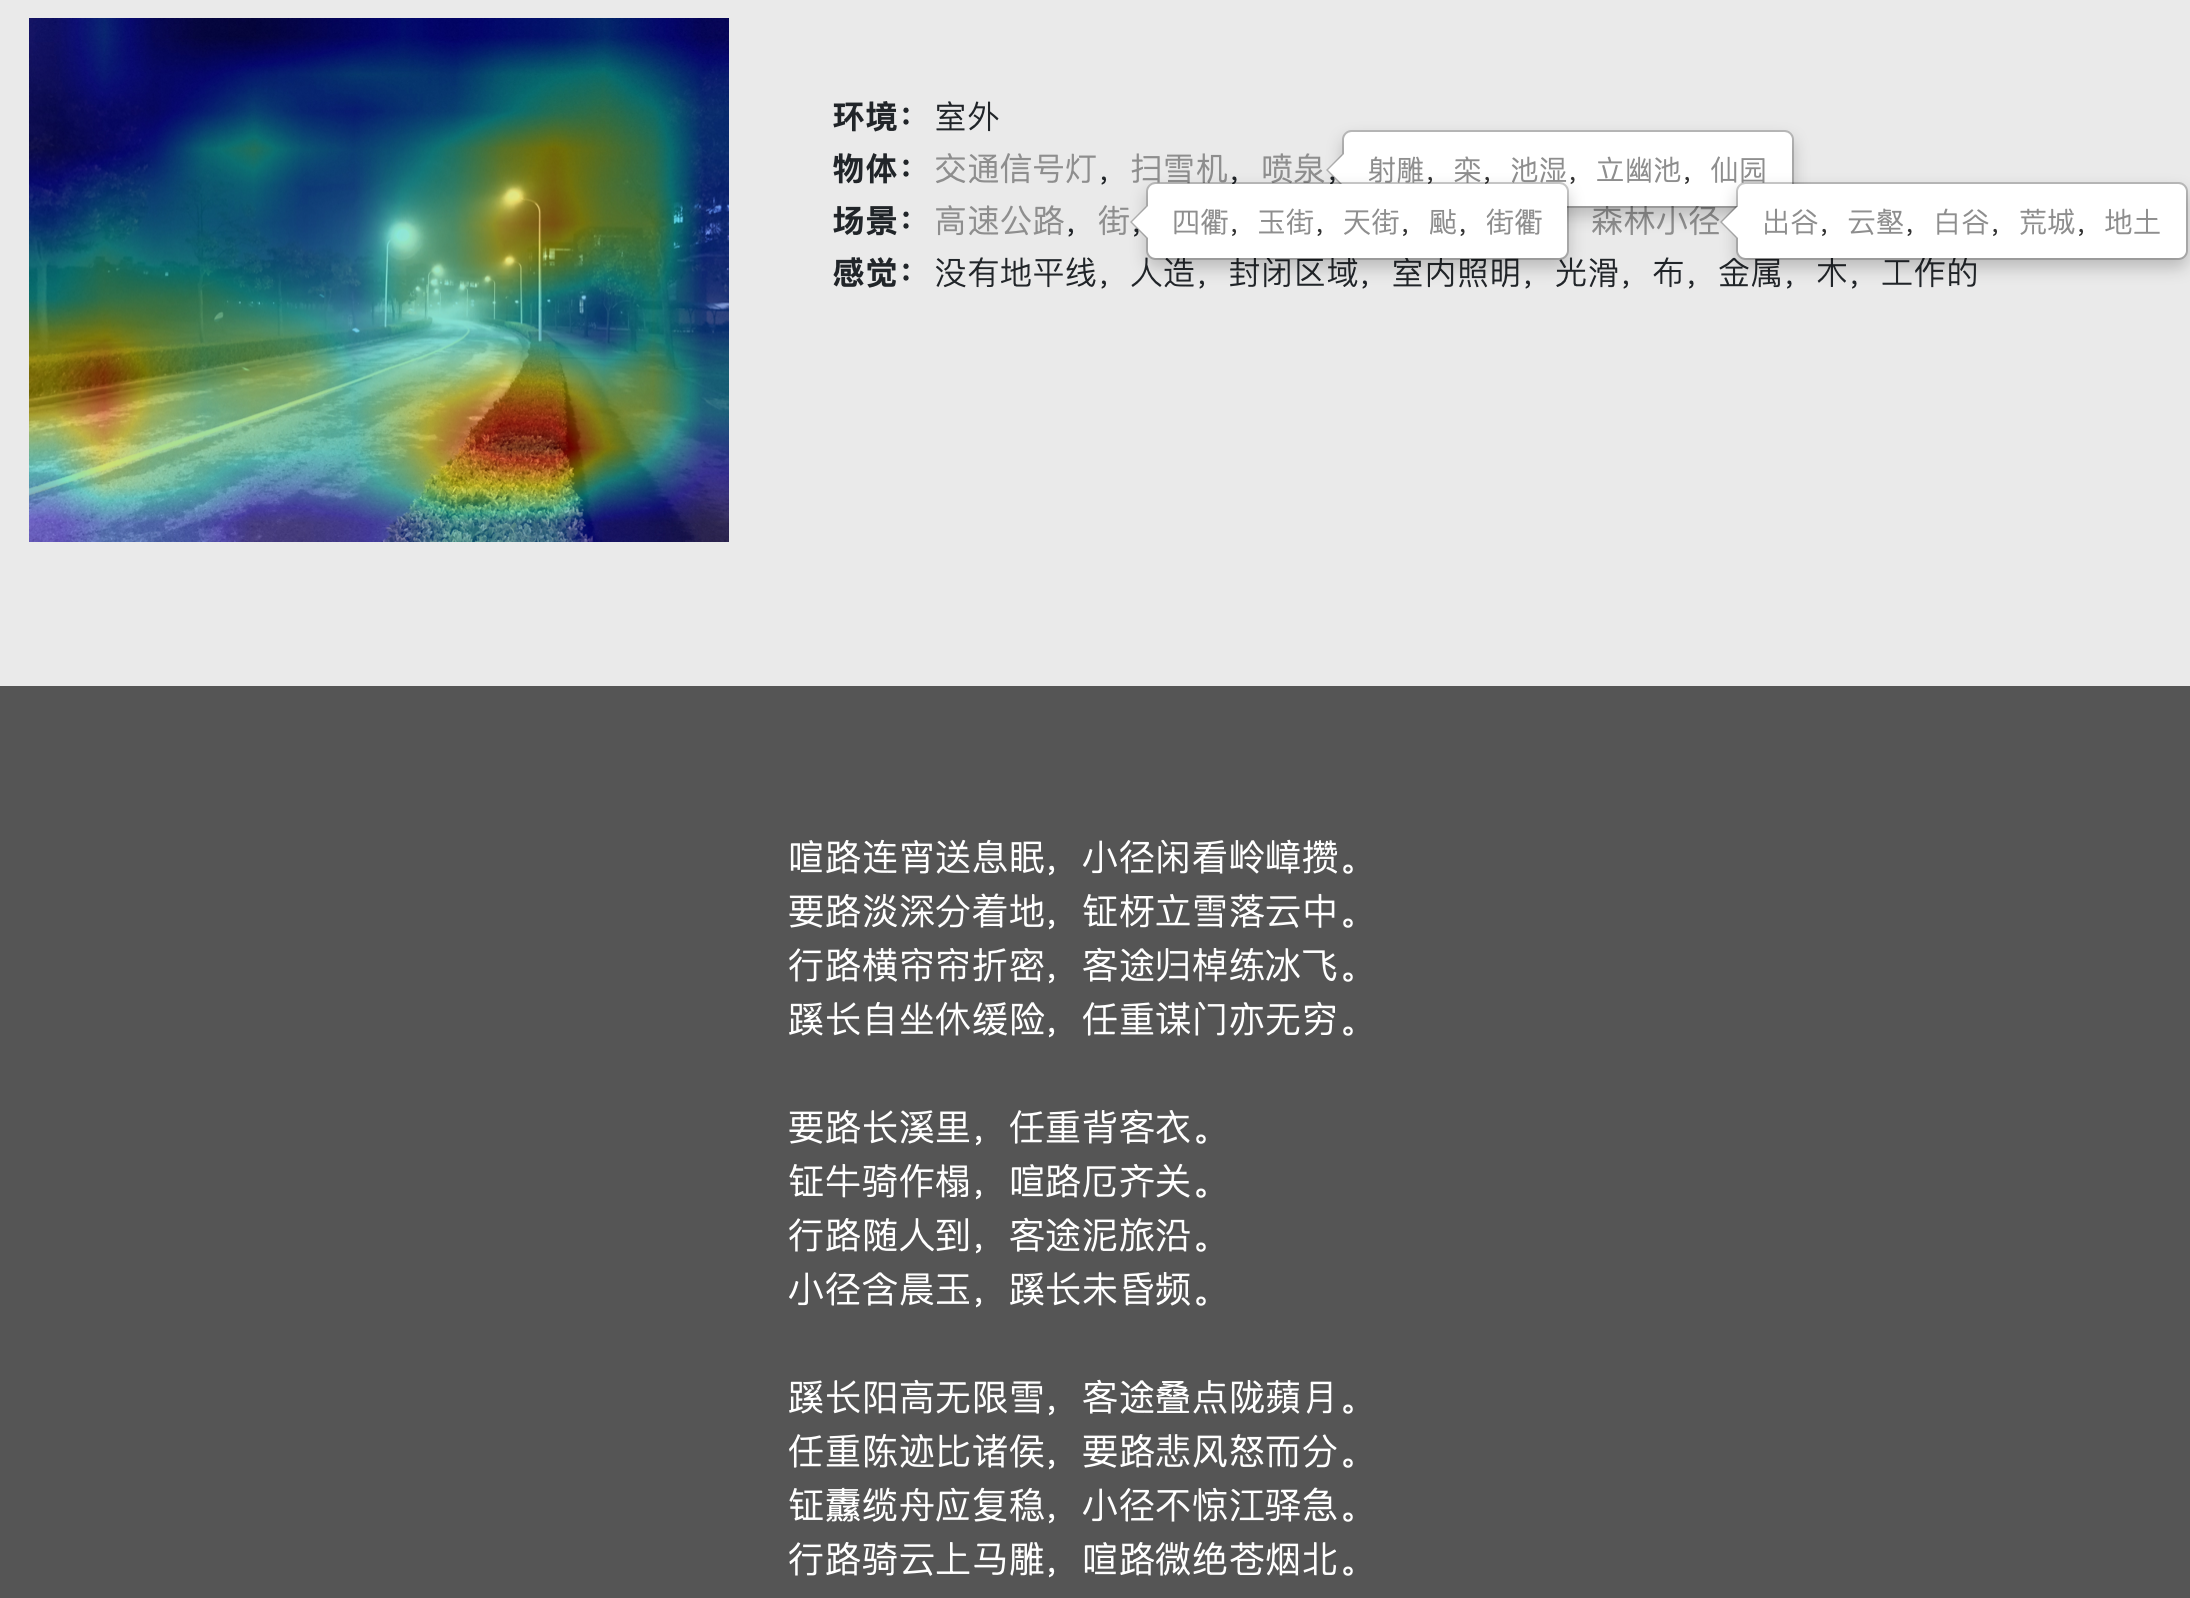
\includegraphics[width=0.9\linewidth]{imgs/7.png}
\caption{从电院草坪夜路生成诗歌}
\end{figure}

在2 GHz Intel Core i5的Macbook Pro上测试,平均每首诗生成时间0.1s,可以接受。

\subsection{现代诗生成}
\subsubsection*{多对抗训练模型}
现代诗的生成我们没有自己训练模型,而是直接参考了来自京都大学和微软亚研院的ACM MM2018的最佳论文\href{https://arxiv.org/pdf/1804.08473.pdf}{Beyond Narrative Description: Generating Poetry from Images by Multi-Adversa},并使用了该论文的开源模型。致谢!

在数据准备上,该现代诗生成模型的数据集分为小部分的多模态诗集(诗+图)和大量的单模态诗集(仅诗),为了扩大有效的多模态数据集,作者首先研究了使用图像CNN特点的deep coupled视觉-诗意嵌入模型,然后利用这一嵌入模型,在单模态诗集中队特征点检索,得到扩大的多模态数据集。
\begin{figure}[H]
\centering
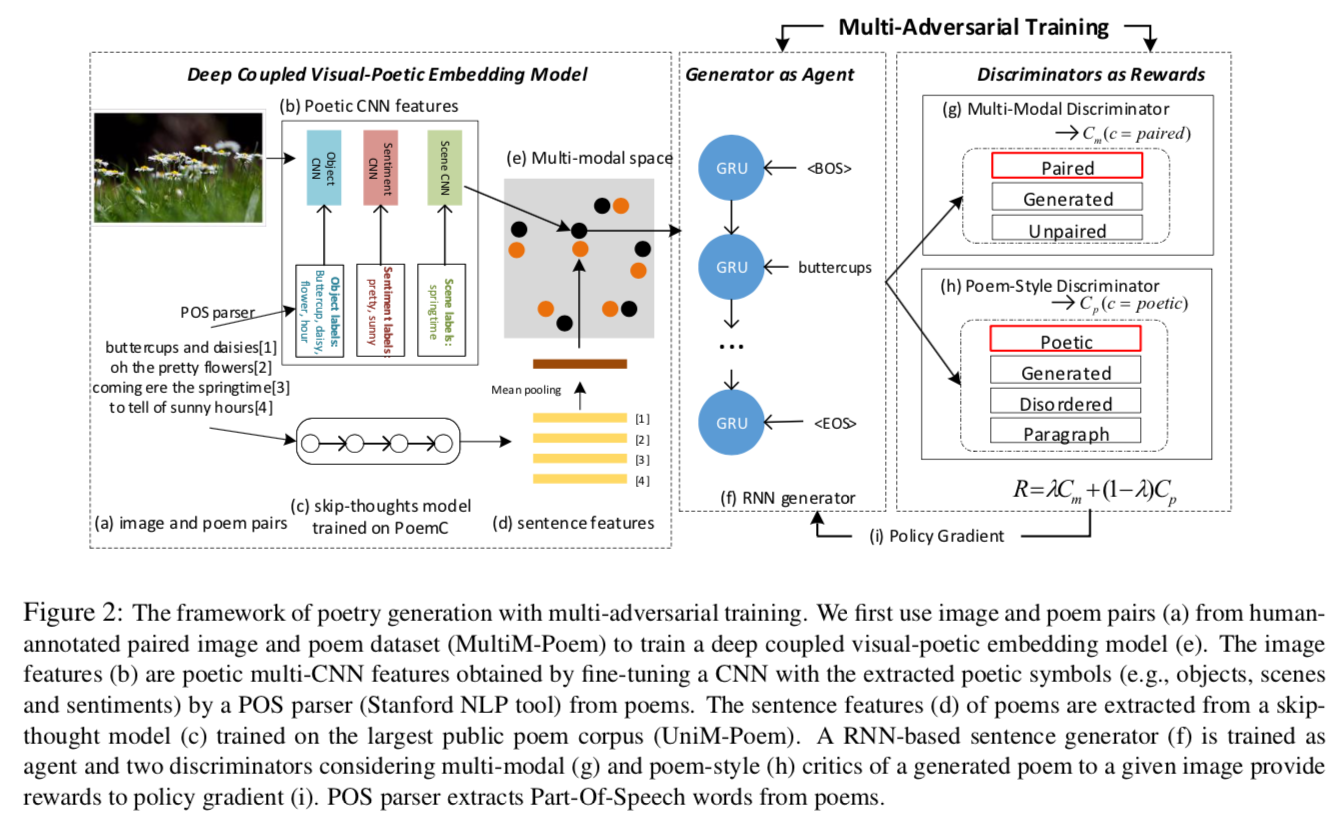
\includegraphics[width=0.9\linewidth]{imgs/8.png}
\caption{该网络的架构}
\end{figure}

在训练上,该模型同样分为两个步骤,提取特征和由特征生成诗歌。提取特征首先由三个cnn得到特征,利用deep coupled视觉-诗意嵌入模型,将空间中不同模态的点进行映射,并使用了图像标注叙事技术,认为一对图像和诗歌共享相同的诗歌语义,则诗与图可用诗歌向量来计算关联。而由特征生成诗歌的步骤,采用策略梯度优化的多对抗训练,同时训练来自人工标注的诗-图正确数据集和生成器等不匹配或无序的负面数据集,两个分别针对诗-图匹配和诗歌风格的判别器以RNN为基础,为策略梯度提供激励。

在我们的实际使用上,由于提取特征利用了三个vgg16网络分别得到图片的物品、场景与情感特征,和我们的图像分析步骤相同,为了节省时间,在前序步骤中我们直接hook并传递了最后一个relu层的4096维输出到生成器中。原网络输出的英文诗,我们经过前面写的抓包爬虫,利用谷歌翻译翻译为英文。
\begin{figure}[H]
\centering
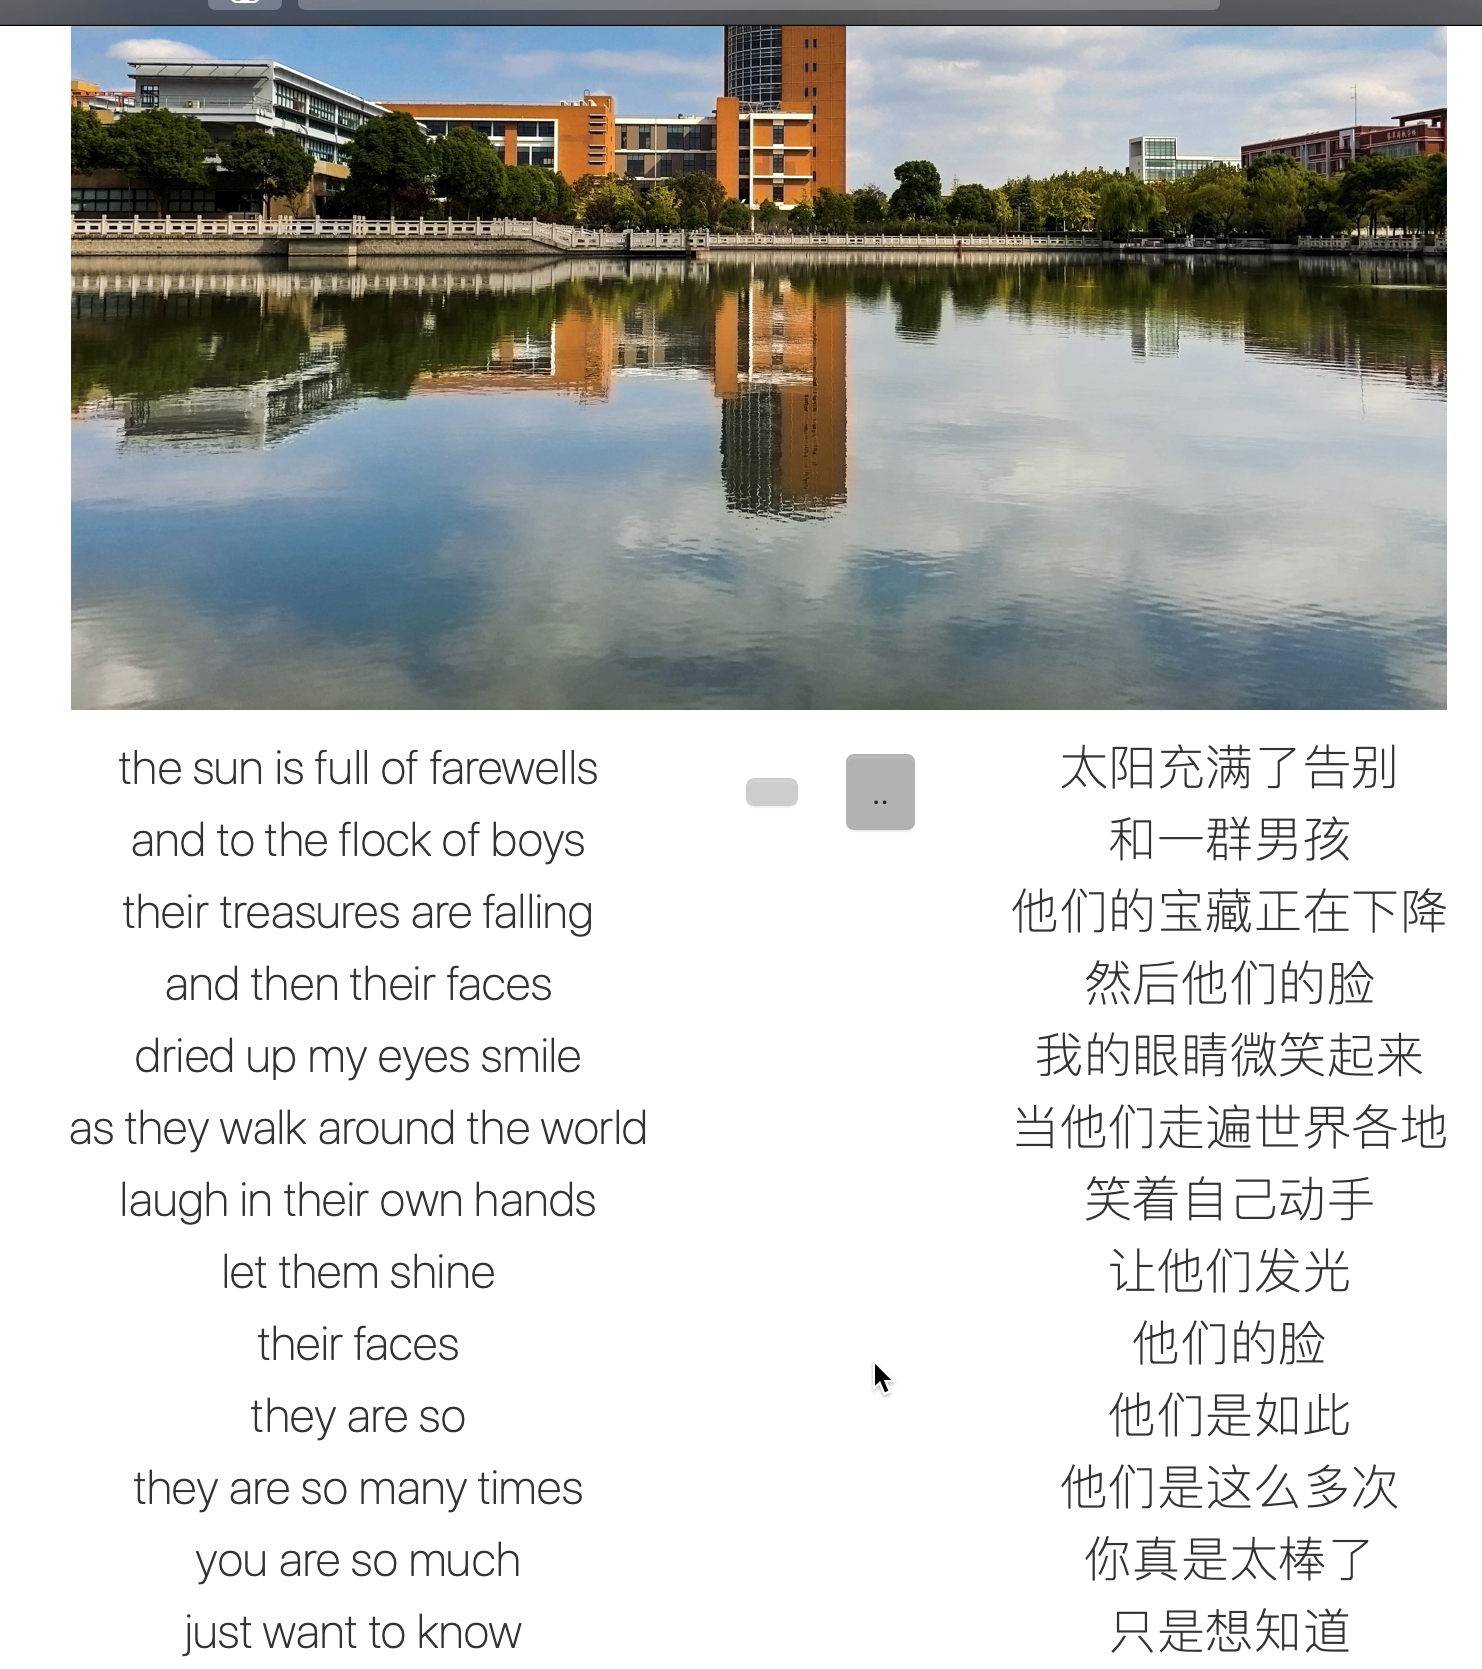
\includegraphics[width=0.7\linewidth]{imgs/9.png}
\caption{从交大图书馆生成现代诗}
\end{figure}

\section{总结}
在本次项目中,我们充分发挥了在实验课上学到的爬虫知识、文本分析索引知识、搜索引擎架构知识,对于图像处理部分,我们未能用上太多课上的知识,但积极探索使用前沿深度神经网络进行图像分析和建立图片与文本间的联系。能够着手构建初具规模,且有一定实用价值的搜索引擎加深了我们对课上知识的认识,并将之付诸实践,我们的实践能力、代码能力以及团队合作能力都得到了一定提升。

以上便是本组报告的全部内容。


\begin{appendices}
\section{项目分工}
数据的爬取由小组成员合作完成,工作量较为平均。

陈浩平\quad 517030910369:索引的创建和更新、文学顾问

李竞宇\quad 517030910318:索引的创建和更新、图片搜索与配图

王中烨\quad 517030910353:前端页面,后端文本搜索,网站前后端衔接

戴昊悦\quad 517030910288:索引的创建、文本语料分析、神经网络模型的设计与训练

\section{项目地址}
以下是我们项目在GitHub仓库上的链接:\href{https://github.com/BruceZoom/EECourse-Poem-Project}{https://github.com/BruceZoom/EECourse-Poem-Project}

\end{appendices}

\end{document}